\documentclass[%
        paper=a4,
	% BCOR=10mm, % Binding CORrection
	oneside,			% two sided printing
        %cleardoublepage=empty,         % empty backsides for two sided printing
        twocolumn=false,
	titlepage=false,			% support for title environment
        abstract,
	numbers=noenddot,		% numbers (in headlines) without ending points
	headsepline,			% line below header
	%footsepline,			% line above footer
	headings=normal,                % size of header is normal
	fontsize=11pt,			% fontsize in points
	pagesize=pdftex,		% define typearea for pdftex usage
        headheight=46.96317pt,          % value based on MyThOS logo
        parskip=off                     % or half*
]{scrartcl}

% ------------------------------------------------------------------------------
% character encoding and fonts for the document
\usepackage[T1]{fontenc} % should be loaded before inputenc
\usepackage[utf8]{inputenc}	    % unicode, newer than utf8x
\usepackage{ae}
\usepackage{aecompl}
\usepackage[T1]{url}			% web adresses with t1 style
\urlstyle{tt}					% web adresses in tt-style
%\usepackage[UKenglish]{babel}
\usepackage[ngerman,UKenglish]{babel}

% ------------------------------------------------------------------------------
% font setup
\usepackage{microtype}
\usepackage{ellipsis}			% corrects wrong spaces after dots
\usepackage{amsmath}
%\usepackage{amsfonts}
\usepackage{amssymb}
\usepackage{latexsym}
\usepackage{dsfont}
\usepackage{textcomp}

%% bera mit euler
\usepackage{bera,amssymb,eufrak}
\usepackage[euler-digits,euler-hat-accent]{eulervm}

\setlength{\parskip}{0.5em plus 1em minus 0.5em}
\clubpenalty 2000
\widowpenalty 2000
%\setlength{\tolerance}{2000}
\setlength{\emergencystretch}{20pt}   % kann man evtl. auf 20 erhöhen
%\setlength{\hfuzz}{1pt}
\setlength{\hfuzz}{10pt}

% ------------------------------------------------------------------------------
% pdf creation
\usepackage[%
  pdftex,
  colorlinks=true,
  urlcolor=red,
  citecolor=red,
  linkcolor=red,
  bookmarks=true,
  breaklinks=true
]{hyperref}

% ------------------------------------------------------------------------------
% graphics
\usepackage{siunitx}
\sisetup{scientific-notation = true}%
\usepackage[usenames,dvipsnames]{xcolor}
\usepackage{graphicx}
\usepackage{subfigure}
\usepackage{tikz}
\usetikzlibrary{calc,trees,positioning,arrows,chains,shapes.geometric,%
    decorations.pathreplacing,decorations.pathmorphing,shapes,%
    matrix,shapes.symbols}
\usepackage{pgfplots}
\pgfplotsset{compat=newest}
\usetikzlibrary{pgfplots.statistics} % For Box plots
\usepgfplotslibrary{units} % Allows to enter the units nicely


% ------------------------------------------------------------------------------
% listings
\usepackage{listings}		% include listings
\newcommand{\code}{\lstinline}
\lstloadlanguages{C++}
\lstset{
  basicstyle=\ttfamily\footnotesize,
  keywordstyle=\bfseries,
  stringstyle=\textit,
  emphstyle=\textit,
  commentstyle=\textit,
  breaklines=true,
  breakatwhitespace=true,
  breakautoindent=true,
  morekeywords={},
  numbers=left,
  numberstyle=\tiny\color{black},
  stepnumber=1,
  numbersep=5pt,
  tabsize=2,
  showspaces=false,
  showstringspaces=false,
    xleftmargin=17pt, 			% left margin where linenumbers and frames do start
    framexleftmargin=17pt, 		% left margin of frame (which will be colored)
    framesep=0pt,
    belowcaptionskip=0pt,
    captionpos=b,
    framerule=1pt
}

\usepackage{scrhack}
\usepackage{float}
\floatstyle{plain}
\newfloat{listing}{tbhp}{myc}
\floatname{listing}{Listing}

% ------------------------------------------------------------------------------
% tables
\usepackage{multirow}
%\usepackage{ragged2e}
\usepackage{tabularx}
\usepackage{longtable}
\usepackage{booktabs}   % toprule, midrule in Tabellen
\newcolumntype{Y}{>{\raggedright\arraybackslash}X}
\usepackage{caption}

\usepackage{collcell}
\newcolumntype{L}{>{\collectcell\lstinline}l<{\endcollectcell}}
\newcolumntype{R}{>{\collectcell\lstinline}r<{\endcollectcell}}

\usepackage{bytefield}

%------------------------------------------------------------------------------
\usepackage{xspace}
\newcommand{\mythos}{\textsc{MyThOS}\xspace}
\def\cc{{C\nolinebreak[4]\hspace{-.05em}\raisebox{.4ex}{\tiny\bf ++}}}

\usepackage[textsize=tiny]{todonotes}

%\usepackage{titling}
\usepackage{enumerate}
\usepackage{epigraph}
\renewcommand{\epigraphsize}{\footnotesize}
\setlength{\epigraphwidth}{0.618\textwidth}
\usepackage{placeins}

\titlehead{
\begin{center}
  \noindent\rule{1.0\textwidth}{1pt}\\[1cm]
  
\includegraphics[scale=0.5]{MyThOS_Logo}\\[0.5cm]
  \sffamily
  \small
  \begin{tabularx}{\textwidth}{lX}
    Förderkennzeichen: & 01IH130003 \\
    Vorhabensbezeichnung: & MyThOS \\
    & Modulares Betriebssystem für Massiv Parallele Anwendungen
  \end{tabularx}\\[0.5cm]
  \noindent\rule{1.0\textwidth}{1pt}
\end{center}
%\vspace{1cm}
}


\usepackage{scrlayer-scrpage}
\makeatletter
\title{\@myTitle}
\renewcommand*{\title}[1]{\def\@myTitle{#1}}
\setkomafont{pageheadfoot}{\sffamily\small}
\lohead{%
\@myTitle\\%
\headmark%
}
\cohead{}
\rohead{
\includegraphics[height=1.5cm]{MyThOS_Logo}}
\makeatother
\pagestyle{scrheadings}

%\usepackage{showframe}

% ------------------------------------------------------------------------------
% layout
\usepackage{multicol}
\usepackage{marginnote}
\renewcommand*{\marginfont}{\footnotesize}
\typearea[current]{last}		% recalculate type area


\title{MyThOS D2.2 Gesamtarchitektur}
\author{Stefan Bonfert, Vladimir Nikolov, Robert Kuban, Randolf Rotta}

\hypersetup{
  pdftitle={MyThOS D2.2 Gesamtarchitektur},
  pdfsubject={MyThOS Deliverable},
  pdfauthor={Stefan Bonfert, Vladimir Nikolov, Robert Kuban, Randolf Rotta},
  pdfkeywords={MyThOS} % comma separated
}

\begin{document}
\selectlanguage{ngerman}
\maketitle

\begin{abstract}
Dieses Dokument gibt einen Überblick über die Gesamtarchitektur des MyThOS 
Betriebssystems, grundlegende Abstraktionen und dynamische Interaktionen. Es 
fasst die Ergebnisse des Arbeitspakets 2 zusammen und erweitert die initiale 
Gesamtarchitektur aus Deliverable D2.1. Dieser Text basiert auf Auszügen aus 
der Kerneldokumentation und ist daher pragmatisch auf Englisch verfasst. 
\end{abstract}

\newpage
\tableofcontents
\newpage
% --- content ------------------------------------------------------------------

\section{Zusammenfassung}

Die Beschreibung der Gesamtarchitektur folgt dem 4+1 Sichtenmodell von 
Kruchten~\cite{kruchten19954+}. Abschnitt~\ref{sec:global-application-view} 
rekapituliert die wichtigsten Anforderungen aus Anwendungssicht. Die Logische 
Sicht (Abschnitt~\ref{sec:global-logical-view}) beschreibt grundlegende Dienste 
und Designelemente zur Umsetzung der funktionalen Anforderungen. Die Physische 
Sicht (Abschnitt~\ref{sec:global-physical-view}) beschreibt die Platzierung und 
Verknüpfung der Systemkomponenten in Bezug auf Speicherbereiche, logische 
Addressräume und räumliche Verteilung über Prozessoren, Kerne und 
Hardwarethreads. Die Dynamische Sicht 
(Abschnitt~\ref{sec:global-dynamical-view}) fokusiert sich auf die 
Interaktionen innerhalb des Kernels und mit Anwendungen, sowie die Verwaltung 
der Lebenszyklen der Systemkomponenten. Die Entwicklungssicht 
(Abschnitt~\ref{sec:global-development-view}) beschreibt grundlegende 
Umsetzungsaspekte in Hinblick auf die nicht-funktionalen Anforderungen.

\paragraph{Anwendungssicht:}
Aus Anwendungssicht ist die Fokussierung auf Vielkern-Prozessoren und hoch-dynamische Szenarien hervorzuheben. Daraus folgt zum Einen der Anspruch möglichst guter Skalierbarkeit der Systemoperationen, das heißt der parallele Durchsatz über viele gleichzeitig aktive Prozessorkerne ist wichtiger als die Latenz einzelner Operationen in Isolation. Zum Anderen wird die dynamische Verwaltung und Konfiguration von Anwendungsthreads und Schutzräumen sowie die Kern-übergreifende Koordination durch parallele Laufzeitumgebungen und (Cloud-)Supervisoren benötigt.

\paragraph{Logische Sicht:}
Die Softwarearchitektur besteht aus vier operativen Schichten: Die \emph{Synchrone Schicht} entspricht der programmiersprachlichen Ebene und besteht aus gewöhnlichen Objekten mit synchronen Methodenaufrufen. Hier werden grundlegende Hardwareschnittstellen und die Ausführungsumgebung für die höheren Schichten bereitgestellt. Die \emph{Asynchrone Schicht} definiert sich über einen Mechanismus für asynchrone Methodenaufrufe. Diese ermöglichen die verzögerte Ausführung zur Umsetzung von wechselseitigem Ausschluss sowie der Delegation zwischen Prozessorkernen. In dieser Schicht sind die Interaktionen zwischen den Kernelobjekten implementiert. Die \emph{Verwaltungsschicht} setzt Zugriffsrechte von Anwendungen auf Kernelobjekte, schwache Referenzen zwischen Kernelobjekten und die Verwaltung der Speicherressourcen um. Hierfür wird ein Ressourcen-Vererbungsbaum in Kombination mit Objekt-Capabilities~\cite{Miller2005} verwendet. Darüber liegt die \emph{Benutzerschicht} mit Anwendungen, Supervisoren und Systemdiensten. 

Als Schnittstelle zwischen Benutzerschicht und dem Betriebssystemkernel fungieren \emph{Kernelobjekte}
orthogonal zu den Softwareschichten. Diese stellen Abstraktionen für Kontrollflüsse, Addressräume, Rechteräume, Hardwarethreads und Kommunikationsportale zur Verfügung. Ein wesentlicher Aspekt ist, dass alle Kernelobjekte explizit über Systemaufrufe aus Speicherpools (\emph{Untyped Memory} Kernelobjekte) erzeugt werden und ansonsten keine dynamische Speicherverwaltung im Kernel notwendig ist. Durch die Partitionierung dieser Speicherpools liegt die Parallelisierung der Systemoperationen sowie die Zuweisung von Resourcen vollständig in der Kontrolle der Benutzerschicht.  

\paragraph{Physische Sicht:}
Die räumliche Positionierung von Aktivitäten erfolgt auf der Benutzerschicht 
und der Asynchronen Schicht. Die Benutzerschicht hat Zugriff auf Kernelobjekte 
(\emph{Scheduling Context}) die die jeweiligen Hardwarethreads bzw. 
Prozessorkerne repräsentieren. Kontrollflüsse werden explizit einem solchen 
Kontext zugeordnet, was der Threadaffinity in anderen Betriebssystemen 
enstspricht. Über Kommunikationkanäle können Anwendungen und Supervisor mit 
gemeinsamen Systemdiensten und mit externen Diensten kommunizieren. Zu den 
externen Diensten gehört zum Beispiel das Lesen und Schreiben von Dateien. 

Auf der Asynchronen Schicht besitzt jeder Hardwarethread einen lokalen FIFO Scheduler für die verzögerte Ausführung der asynchronen Methodenaufrufe. Kernelobjekte werden entweder bei ihrer Erzeugung an einen Scheduler gebunden, was den Ausführungsort aller ihrer Aktivitäten statisch festlegt, oder der Ort wird über einen Delegationsmechanismus dynamisch ausgewählt, wobei wechselseitiger Ausschluss auf dem Objekt gewährleistet bleibt. 

Die logischen Adressräume sind unterteilt in einen festen, gemeinsamen 
\emph{Kernel Space} und einen konfigurierbaren \emph{User Space} für die 
Benutzerthreads. Die Adressabbildungen für den Kernel Space sind in das Image 
eingebettet, um direkt nach dem Start des Prozessors zur Verfügung zu stehen 
und werden später nur minimal verändert. Im Kernel Space gibt es einen Bereich 
in den die ersten 4GiB des physischen Addressraums direkt eingeblendet sind. 
Dieser Bereich wird für alle späteren Kernelobjekte verwendet und die Größe 
ist so gewählt, dass selbst auf 64-bit Systemen mit kompakten 32-bit Zeigern 
gearbeitet werden kann.

\paragraph{Dynamische Sicht:}
Um eine gute parallele Skalierbarkeit zu ermöglichen erscheint es sinnvoll, 
dass mehrere Anwendungsthreads nebenläufig Systemaufrufe durchführen können. 
Aufgrund der sehr beschränkten Speicherressourcen sollten durchsatzunkritische 
Kernelobjekte gemeinsam benutzt werden, um den Replizierungsoverhead zu 
vermeiden. Dafür müssen Zugriffe auf gemeinsam genutzte Kernelobjekte 
koordiniert und synchronisiert werden. Tasklet-basierte Monitore in den
Kernelobjekten ordnen die Ausführung asynchroner Methodenaufrufe um
wechselseitigen Auschluss sicher zu stellen. Durch ineinander verschachtelte
asynchrone Aufrufe sind prinzipiell Deadlocks möglich, da dies verschachteltem
Locking entspricht. 
Dem kann nur auf architektureller Ebene durch asymmetrische Rollenverteilung 
zwischen den Kernelobjekten begegnet werden.  

Ein weiterer wichtiger Aspekt ist die koordinierte Löschung von Kernelobjekten. 
Dies geschieht in drei Phasen. Zuerst werden über den Ressourcen-Vererbungsbaum 
alle Langzeit-Referenzen (beschrieben durch Objekt Capabilities) zurückgezogen. 
Dann wird mittels eines asychronen Broadcasts über alle gerade im Kernel 
aktiven Threads sichergestellt, dass keine unsichtbaren temporären Referenzen 
in Registern u.ä.übrig sind. Anschließend wird die finale Löschung des Objekts 
asynchron verzögert, bis der Referenzzähler für temporäre Referenzen Null 
erreicht hat.

\paragraph{Entwicklungssicht:}
Um eine modular konfigurierbare Systemarchitekur zu erreichen, wird das Prinzip der \emph{Dependency Injection} auf mehreren Ebenen eingesetzt. Anstelle von Anfragen an zentrale Verzeichnisse oder der Speicherallokation aus zentralen Pools bekommen Kernelobjekte alle notwendigen Abhängigkeiten bei ihrer Erzeugung bzw. später über Konfigurationsmethoden von außen mitgeteilt. Das Selbe gilt für die statische Auswahl von Implementierungsvarianten über C++ Template Mechanismen. Auf der Ebene des Quellcodes entspricht dieses Prinzip der Komposition der finalen Software aus Code-Modulen. Abhängigkeiten werden durch die Verwendung entsprechender Header-Dateien deklariert und mit Hilfe des mcConf Werkzeugs wird eine passende Implementierung aus der Modulsammlung ausgewählt. Im Vergleich zu den Template-basierten Mechanismen ist dies flexibler und resultiert in besser lesbarem Code.  

Der Ressourcen Vererbungsbaum wird lediglich als doppelt verkettete Liste der Knoten in Prefix-Ordnung gespeichert. Dank der 32-bit Zeiger in den 4GiB Kernelspeicher werden so nur 16 Byte pro Eintrag benötigt (entspricht zwei 64-bit Zeigern), um Vorgänger, Nachfolger, Zielobjekt und Metadaten wie Zugriffsrechte zu repräsentieren. Abgeleitete Referenzen werden direkt hinter der ursprünglichen Referenz eingefügt. Zum Zurückziehen von Zugriffsrechten wird der betroffene Teilbaum mittels eines Vaterschaftstests traversiert. Die Implementierung der Baumoperationen ermöglicht voll nebenläufige Aktivitäten auf voneinander unabhängigen Teilbäumen. 



% --- content ------------------------------------------------------------------
\selectlanguage{UKenglish}
\section{Application View}
\label{sec:global-application-view}

The target application domain of MyThOS is dynamic and elastic high-throughput parallel 
computing applications on many-core processors. 
%
For example, complex multi-physics simulation codes exhibit multiple coupled applications operating in turns and in parallel on shared data. \emph{Invasive computing}~\cite{InvasiveComputing,octopos} tackles the difficult load balancing by trading cores dynamically between the individual applications.
%
Similarly, new applications in big data, deep learning, and the internet of things raise the need for \emph{elastic} compute clouds~\cite{Rhoden:2011:IPE:2038916.2038941}. In addition to the dynamic assignment of cores to compute tasks, these scenarios require effective isolation and supervised communication between third-party compute codes.

The requirements from the application's viewpoint divide into three general
types of user-space activities: actual applications that perform computations,
supervisors that globally coordinate between the applications, and basic system
services that provide a shared infrastructure.
The supervisors require mechanisms to exert control over applications such as
assigning and revoking physical memory, storage in general, compute cores, and communication channels.
This includes the ability to preempt and migrate application threads as well as 
to intercept protection violations and similar events. In this way, 
policies such as the mapping of application threads to physical cores and invasive computing~\cite{InvasiveComputing} can be implemented.
Beyond this, the three types share requirements with respect to the management
of threads, address spaces, shared memory, and communication.

Application threads provide logical control flows that are scheduled for 
execution by the operating system and operate in an application-specific 
environment.
Interfaces are needed to create/delete and 
suspend/wakeup application threads.
The thread's execution environment is composed of a logical address space, 
thread-specific data (stack, basic communication buffers, thread-local data) 
inside this address space and access rights to system services and 
communication channels.    
Hence, an interface is needed to map actual memory into these address spaces and configure the processor's support for thread-local data.
On many-core processors, an additional core-local storage relative to 
physical hardware threads seems useful.

Basic communication support by the OS kernel is needed for inter-process communication (IPC) between application, supervisors, and system services, e.g., to communicate requests and set up high-level communication.
If system services are partially implemented by kernel objects instead of user-space threads, a uniform interface is needed to hide the implementation-specific differences.  
High-volume data transfers are usually facilitated via shared memory, which requires means to setup shared memory across address spaces.
In this context, asynchronous and optionally preemptive notification mechanisms
are useful in order to avoid busy polling on shared message buffers.
The actual communication between application threads is up to the application's parallel programming runtime. 

\section{Logical View}
\label{sec:global-logical-view}

This section describes the logical view, which consist of common services, mechanisms, and design elements that fulfill the functional requirements of the system.

From the application's point of view, abstractions for communication with the operating system services, for communication with other applications, and for the management of their execution environment are needed. These abstractions define the overall system's style and versality.
For example, Unix-based systems expose a large number of kernel functions via the system call interface. Where a reference to a specific instance, for example a file, is needed, a numeric handle, for example a file descriptor, is passed via the call arguments and the kernel function looks up the instance in a type- and process-specific table.
Other designs focus directly on these instances and let the application communicate with them via a small set of system calls, see for example~\cite{Liedtke1996}. This style is closer to method invocations on kernel objects. A major advantage is, that the management of instances can be unified while giving the application/user more explicit control.

\subsection{Layers and Object Types}
\label{sec:vert-layer}
% problem statement
Different styles of interaction between objects can be found inside the kernel. This is caused by the differentiation between purely local actions that do not leave their hardware thread, communication mechanisms that coordinate the kernel's activities across hardware threads, and the communication between user-mode applications and kernel via system calls and invocation messages.

This section introduces layers of the software architecture in order to simplify the later discussion of the respective interaction styles. The interaction styles also constrain the object model in order to lead to interoperable interfaces. A short summary of the layers and object models in shown in Figure~\ref{fig:layers}.

\begin{figure}
  \centering
  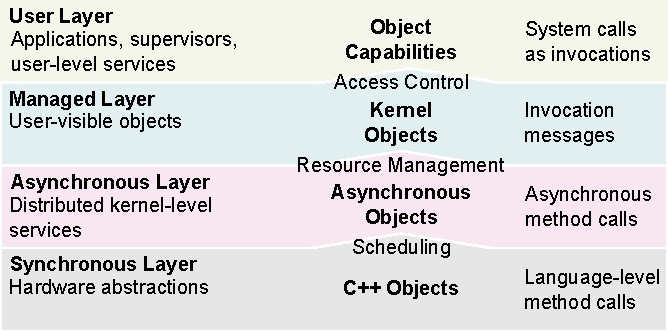
\includegraphics[scale=1]{fig/layers.pdf}
  \caption{Layers and object types.}
  \label{fig:layers}
\end{figure}

\begin{description}

\item[Synchronous Layer:] This is the lowest, most basic layer of the architecture. Ordinary \emph{C++ objects} are used to implement fundamental data structures and basic hardware abstraction components. These objects are used via the ordinary C++ method and function calls and their implementation is executed immediately in the current logical control flow.

This layer is responsible to provide the runtime environment that is needed by the asynchronous layer. This includes the scheduling of asynchronous activities across hardware threads and mechanisms for concurrency and locality control. \emph{Tasklet} objects provide the abstraction for asynchronous activities and \emph{monitor} objects implement asynchronous synchronisation policies such as mutual exclusion.

\item[Asynchronous Layer:] On top of the runtime environment from the synchronous layer, this layer hosts \emph{asynchronous objects} that provide communication via asynchronous method calls. In contrast to arbitrary C++ object methods, the asynchronous methods consume a Tasklet as small state buffer and a reference to an asynchronous response handler object. The actual implementation of the called method can be executed at a later time and also on a different hardware thread. The call returns by calling a respective asynchronous response method, passing along the Tasklet. 

This layer implements shared kernel infrastructure and is not directly visible to the user. Examples are the \emph{resource inheritance tree} and supporting asynchronous objects for the implementation of kernel objects.

\item[Managed Layer:]
\marginnote{See also~\ref{sec:capability-impl}}
This layer manages the resources and life cycle of \emph{kernel objects} through \emph{capabilities} as an unified smart pointer mechanism. The capabilities track the resource inheritance beginning from memory ranges over kernel objects allocated in this memory to derived weak references that point to the same kernel object. In cooperation with the memory management this inheritance enables the clean deallocation of kernel objects and recycling of the respective memory. 
Alongside the basic state information that is used by the kernel's resource management, the capabilities include generic and type-specific access rights. These are used by the system call interface to restrict the user's capability invocations. Such invocations are forwarded as asynchronous method call's to the \emph{invoke()} method of the targeted kernel object.

This layer contains all user-visible and call-able system services, which are introduced in Section~\ref{sec:kernel-objects}. A small set of system calls allows to push capability invocations from the application to the kernel objects.

\item[Application Layer:] Applications, supervisors, and other system services live in the application layer. Application threads interact with \emph{kernel objects} via \emph{capability pointers}, which are logical indexes into the thread's capability space. Communication on the application layer is possible via shared memory in the logical address spaces and via inter-process communication (IPC) services of the kernel. Libraries can introduce various middleware layers for higher-level parallel abstractions.
\end{description}

\subsection{Core Abstractions: Kernel Objects}
\label{sec:kernel-objects}

\begin{figure}
  \centering
  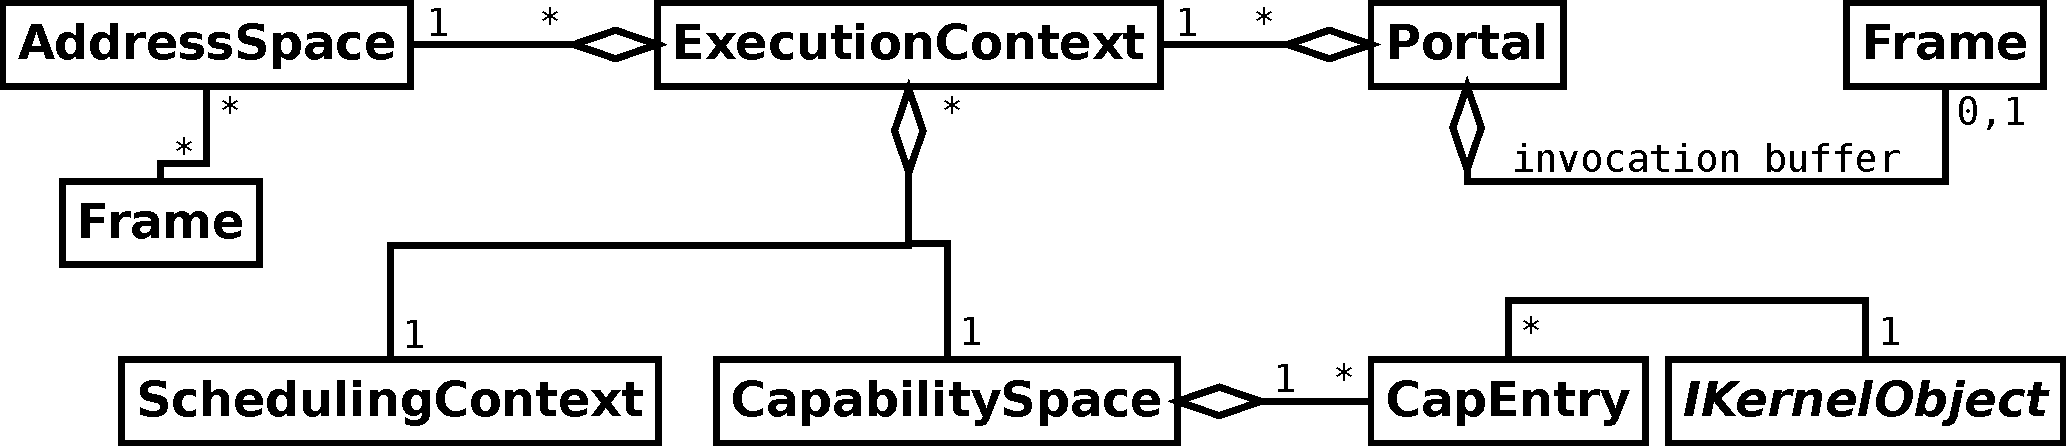
\includegraphics[scale=0.25]{fig/kernel-objects-logical.pdf}
  \caption{Interaction between the basic kernel objects.}
  \label{fig:kernel-objects-logical}
\end{figure}

\emph{Kernel objects} are the smallest components with a managed and application-visible life cycle. Figure~\ref{fig:kernel-objects-logical} shows a class diagram of the interactions between the core kernel objects. 

\begin{description}
\item[Address Space:]
\marginnote{See also~\ref{sec:address-space-phys}}
The logical address space configuration, that is the translation from logical to physical addresses and the access protection, is represented through Address Space kernel objects. They allow to manipulate the protection flags, map physical memory frames into a logical address space, and unmap address ranges. The Address Space is responsible to react to the deletion of mapped frames, which happens through the resource revocation mechanism and unmaps the frame. The TLB invalidation on all affected hardware threads has to be implemented by the owner of unmapped or revoked frames because the user-level code has to keep track of the used address spaces anyway.

\item[Capability Space:] These manage the application's access to kernel objects by implementing a mapping from numerical capability pointers to capability entries. These entries contain the pointer to the kernel object, meta-data such as access rights, and information about the inheritance history for the resource management.  

\item[Execution Context:] User-mode threads are represented by Execution Contexts. Each execution context is associated with an address space, a capability space, and a scheduling context. It is responsible to track the execution state (waiting, running, preempted\ldots) and the user-mode processor state (register contents, the thread-local storage configuration\ldots). The address space, capability space, and scheduling context can be shared between many threads and arbitrary combinations are possible.

\item[Scheduling Context:]
\marginnote{See also~\ref{sec:locality-control}}
Scheduling contexts manage the processing time of execution contexts on hardware threads. It is their responsibility bring ready execution contexts into actual execution by scheduling them on a selected hardware thread. 
In the basic variant of \mythos, each scheduling context represents a single hardware thread and the associated execution contexts are scheduled cooperatively only on this thread with FIFO order. Thread migration can be achieved by rebinding execution contexts to other scheduling contexts.

\item[Portal:] 
\marginnote{See also~\ref{sec:portal-dyn}}
Portals facilitate the deferred synchronous \emph{communication} between execution contexts as well as between applications and kernel objects. Each execution context needs a portal in order to issue capability invocations, send and receive IPC requests, and send responses. Portals hold a capability to an \emph{invocation buffer} frame, which is used as shared message buffer between application and kernel. Each portal is associated with one execution context, which is resumed whenever a message arrives at the portal.

\item[Frame:] In order to map physical memory into an address space, especially to established shared memory across address spaces, a handle to such physical memory regions is needed. These are represented by frames as contiguous well-aligned ranges of physical addresses. The frame objects are responsible for tracking the memory's use in address spaces and enforce effective revocation by unmapping themselves from all affected address ranges. Frame capabilities can be inherited into subranges of the frame.

\item[Untyped Memory:]
\marginnote{See also~\ref{sec:kernel-space-management}}
Appropriate (physical) memory is needed in order to create new kernel objects. These memory ranges cannot be frames, because this would allow to map the memory of kernel objects into user-level address spaces. Hence, untyped memory is used as origin of the available physical kernel memory. Like frame objects, untyped memory objects represent contiguous ranges of physical addresses. They are responsible to manage the used versus free parts of the range. Resource inheritance is used to split free untyped memory into smaller portions. This is the key ingredient to the user-controlled distributed concurrent allocation of kernel objects. 

Converting untyped memory into actual kernel objects is achieved via factories. The initial factory implementation is responsible for all the basic kernel objects described in this section. The creation of custom, application-specific kernel objects can be facilitated via additional factory kernel objects or by extending the initial factory implementation.
\end{description}

\subsection{Concurrency Control: Tasklets, Monitors, Lock-Free Algorithms}
\label{sec:concurrency_control}

% problem statement
In a system with many concurrently running hardware threads, multiple threads can perform system calls in parallel. This introduces a consistency challenge because one thread could manipulate or delete a kernel object while another thread tries to use it. 
In addition, interrupt signals and traps from the processor and devices can preempt the execution of a hardware thread and jump into kernel mode. Preemption of user-space activities looks very similar to entering the kernel via system calls. But preemption of kernel-mode execution can introduce subtle deadlocks and inconsistencies. 
Hence, a concurrency control strategy is needed that ensures consistency of all kernel state.

% our solution
The \mythos kernel does not allow on-demand allocation. In consequence, no message objects, state copies, or kernel threads can be allocated on the fly. The concurrency control has to operate with statically allocated resources. This excludes unbounded asynchronous messages, read-copy-update mechanisms, and cooperative kernel threads for lock-based critical sections. The kernel should not wait busily in fine grained locks. Event-style execution models can be a useful alternative if all aspects of the system design and implementation respect their limitations and constraints. This has the additional benefit, that single-stack kernels need an event-based model anyway.   

\begin{itemize}
\item All asynchronous operations have to be deferred synchronous cycles. Requests transfer the logical control flow and responses return it.
\item Transitional states and the transitional use of internal resources has to be protected by a flow control mechanism. The next incoming request can be processed just after the all outstanding responses of previous deferred synchronous cycles have been processed.
\item There is just a finite number of entry points into the kernel (system calls and interrupts) and each entry point can initiate just a finite number of logical control flows.
\item Forking of logical control flows requires the ownership of statically allocated resources.
\end{itemize}

In MyThOS, \emph{asynchronous objects} are the main synchronisation mechanism throughout the kernel, providing mutual exclusion, operation ordering, flow control, and bounded asynchronous communication. These objects provide \emph{asynchronous methods}, which are called like C++ methods but are actually executed later and possibly on a different hardware thread.

\begin{description}
\item[Tasklets:] 
\marginnote{See also~\ref{sec:tasklet-impl}}
The signature of asynchronous methods follows a specific pattern: a reference to a \emph{Tasklet} object is passed as temporary storage for the asynchronous execution state. The Tasklet objects have a fixed structure that enables enqeueing into queues, reflecting about source and destination of the task, and a handler function with a limited space for additional state data or arguments.

\item[Monitors:] 
\marginnote{See also~\ref{sec:locality-control}}
Inside the asynchronous methods, \emph{monitor} objects are used to implement the actual synchronisation and communication. Different variants are available to choose between simple mutual exclusion, multiple reader/single writer, response-before-request synchronisation patterns. The monitors do not need dynamic memory management because they use the forwarded tasklet argument to manage their processing state and communication. 
\end{description}

It is the monitors responsibility to bring enqueued tasks into actual execution on a suitable hardware thread. As example implementation, each monitor is bound to a hardware thread and all Tasklets are enqueued into a task queue at this thread. This ensures mutual exclusion. Priorities like preferring the processing of responses over beginning of new requests can be implemented by a respective priority hierarchy of task queues at each hardware thread. A different implementation, similar to delegation queue locks, uses a Tasklet queue inside the monitor. Whenever a new task is enqueued as first task the hardware thread has mutually exclusive access and can process the task directly or enqueue the monitor into the threads task queue.

\paragraph{Discussion.}
The life cycle of a Tasklet can be interpreted as a credit-based flow control: Client objects can issue asynchronous calls only if they own a currently unused Tasklet, that is have remaining credit. The request call passes the Tasklet credit to the server object and, there, it can be used for further internal asynchronous processing. Finally, the response call returns the Tasklet and the associated credit back to the client, which enables the client to issue a new asynchronous request. 

The Tasklet life cycle can also be interpreted as a logical control flow. The request call forks the logical control flow and the Tasklet is used as message from client to server. Inside the server, the Tasklet stores the logical control flow's state. Finally, the response call finishes the logical control flow and the Tasklet acts as message from server to client.

The monitors are implemented on the synchronous layer where just ordinary synchronous C++ method calls but no mutual exclusion or locking mechanisms are available. Here, synchronisation and communication primitives of the hardware have to be used. For example, atomic compare-and-swap, fetch-and-add, and exchange operations on shared memory are sufficient to implement the obstruction-free FIFO queues needed for the monitors. 

\hspace{0px}\marginnote{See also~\ref{sec:credit-flow-dyn}}
The monitors can be interpreted as actors~\cite{Hewitt:1973:UMA:1624775.1624804} that send Tasklets as messages between each other. Instead of unlimited asynchronous message queues like in actor models, the degree of asynchronous activity is bounded by the limited amount of statically allocated Tasklets. Unlike a fixed-size mailbox for incoming messages, the \mythos Monitor's can receive an unlimited amount of tasklets without failing or blocking.

\subsection{Dynamic Resource Management through Capabilities}
\label{sec:log:capabilities}

% problem statement
One of the main problems that a kernel has to solve is the management of dynamic resources---especially the dynamic allocation and deallocation of objects in the kernel's memory. Which and how much memory is an application allowed to use? What happens if the kernel's memory reserve is depleted? Which kernel objects are affected when deleting an object? When is it safe to delete objects and which are still used by an application?

% our solution
\mythos solves these problems through three principles. First, all kernel objects are designed to operate without any on-demand allocation. For example, the asynchronous communication layer \marginnote{Sec.~\ref{sec:concurrency_control}} pre-allocates all needed message buffers inside the callers of asynchronous objects. Likewise, the IPC portals communicate with pre-allocated invocation buffers. Hence, the system's normal operation is not impacted by hidden memory management overheads and cannot fail due to depleted resources. 

Second, just the creation and deletion of kernel objects involves dynamic memory management. The respective memory pools are represented via Untyped Memory kernel objects. When an application wants to create a kernel object, it first has to own an Untyped Memory capability with sufficient free space. \marginnote{Sec.~\ref{sec:boot-dyn}} The boot sequence hands over the initial Untyped Memory. In combination, this steers the applications' use of kernel memory and using up all memory does not affect unrelated applications.

\begin{figure}
  \centering
  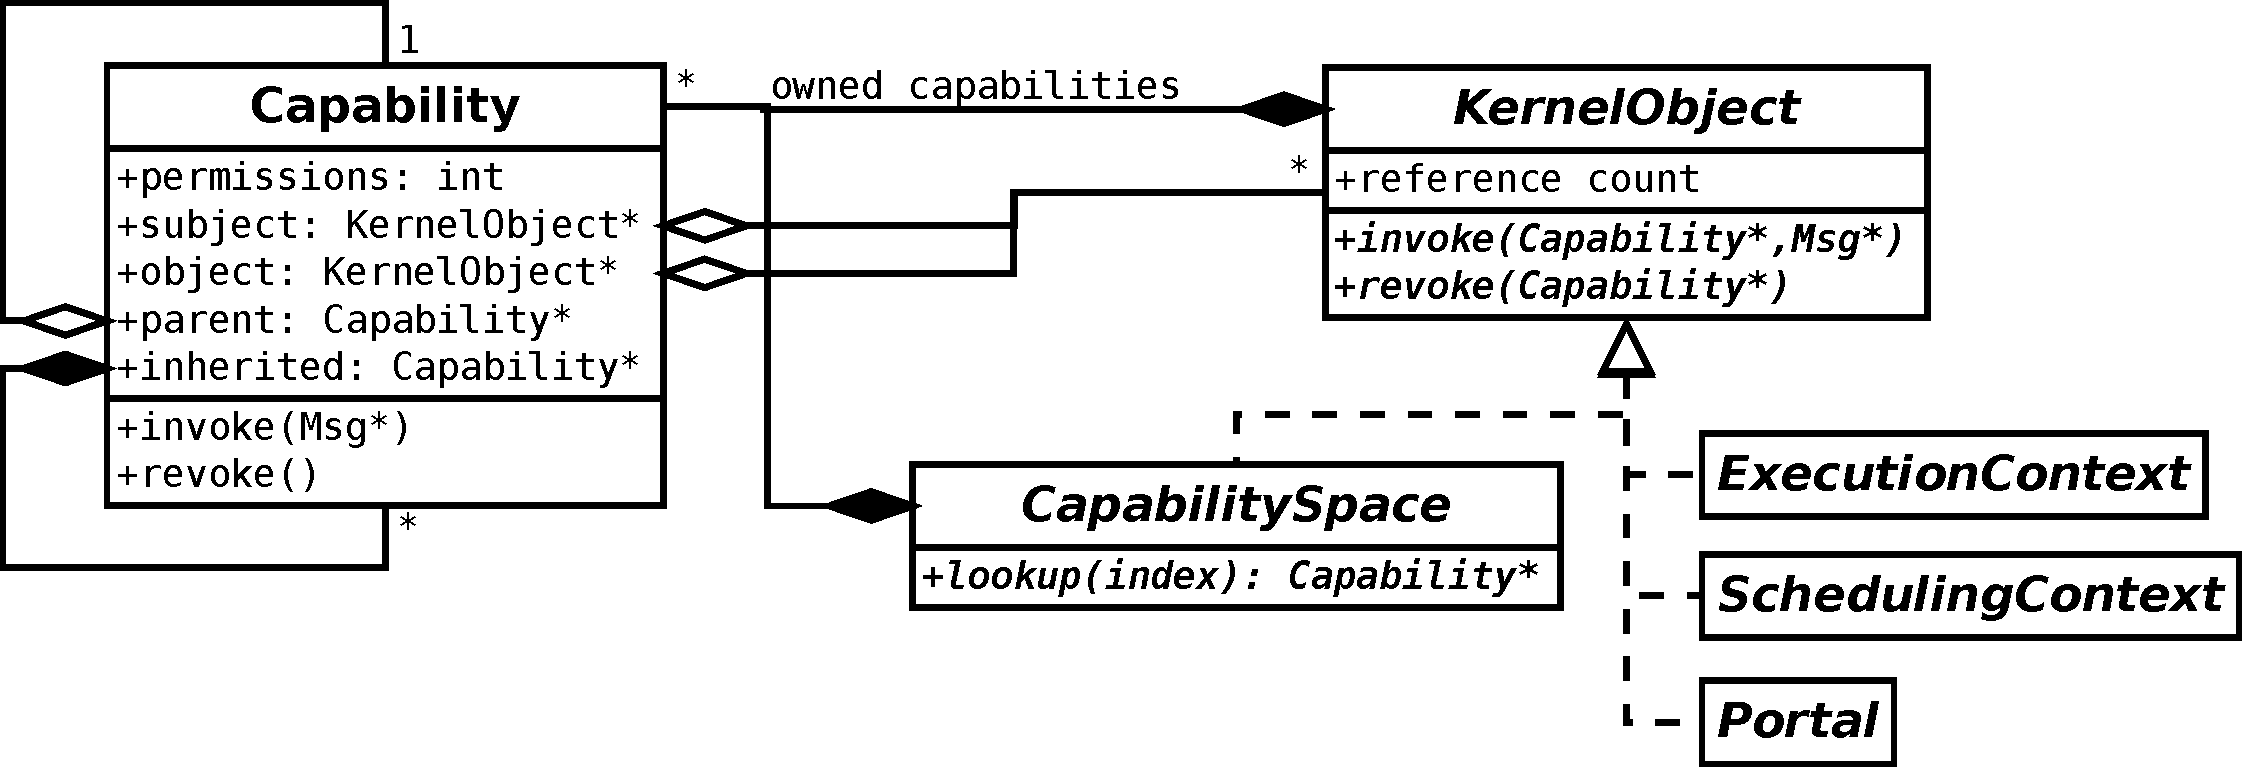
\includegraphics[scale=0.25]{fig/capability-model.pdf}
  \caption{Conceptual interactions between capabilities as smart pointers and kernel objects. The implementation stores just a subset of these pointers.}
  \label{fig:capability-model}
\end{figure}

Finally, based on the concept of object capabilities, the resource inheritance tree implements smart pointers and weak references to kernel objects in combination with tracking the object's resource inheritance. \marginnote{Sec.~\ref{sec:capability-impl}} Figure~\ref{fig:capability-model} shows a conceptual model of the interactions between capabilities and kernel objects. When a kernel object is allocated from an Untyped Memory, a respective Original Capability is created that points to the kernel object and has the Untyped Memory as parent. Therefore, the inheritance tree enumerates all objects that are contained inside the memory region and allows to force the deletion of the contained objects. Likewise, all long term references to kernel objects are stored as children inside the inheritance tree.  

The inheritance acts as a weak reference mechanism with the added benefit of being able to inform the affected subjects about the ongoing deletion. By removing all inherited capabilities, the kernel ensures on behalf of the user that no new asynchronous activities can be started on the object. On top of this mechanism, the deferred deletion support of the asynchronous objects layer ensures that objects are not deleted before all deferred activities have completed.

The capability paradigm of Miller et al.~\cite{Miller2005} differentiates between subjects, objects, permissions, and invocations. 
\emph{Subjects} are the smallest units of computation that can hold access rights and \emph{objects} are the smallest units to which access rights can be provided. 
A \emph{direct access right} gives the subject the permission to invoke the behavior of the object.
In this sense, the kernel objects take the role of capability subjects and objects. 
The user cannot access capabilities directly, that is their instance data structures as C++ object. Instead, a capability space maps from numerical indexes to capability entries. Some capability entries are stored inside other kernel objects and can be used only indirectly. 

\subsection{Physical Memory and Address Space Management}
\label{sec:memory-impl}

Virtual memory with access control is the most important hardware-level protection mechanisms. Thus, any manipulation of the hardware's address translation tables has to be supervised by the operating system. Otherwise, applications might be able to map foreign physical memory into their own address space and compromise the consistency of the overall system. 

The current x86-64 processor architectures support up to three different frame sizes (4KiB, 2MiB, 1GiB) and the address translation employs a four-level page table structure. The following kernel object types are used to represent them:

\begin{description}
\item[Frame:] A frame represents a contiguous range in the physical address space that is backed by some kind of memory or a memory-mapped device. The range is restricted to certain sizes and respective alignment in order to reduce implementation overhead. Currently these are 4KiB, 32KiB, 256KiB, 2MiB, 16MiB, 128MiB, 1GiB, and 8GiB.

It is not useful to dynamically allocate additional kernel objects whenever smaller frames are derived from a large frame. These objects would inherit resources from \emph{both} the original Frame and an Untyped Memory, which violates the resource inheritance tree. Instead, the \emph{flyweight} pattern~\cite{gof} is used, that is Frame capabilities point to the same statically allocated Frame kernel object.

\item[MemoryRegion:] For frames that lie outside of the kernel's initial Untyped Memory, a respective base for the flyweight Frame object is needed. These are allocated as MemoryRegion objects and provide the shared Frame object for all frames that are derived from this region.  

\item[PageMap:] Each page map represents an individual table in an address space structure. Page maps are bound to a specific level during their creation. When mapping a frame or a page map into a page map's entry, the kernel checks the frame size and page map levels. One can map either a page map of the next lower level or a frame of the same level.

The top level table is called \emph{page map level 4} (PML4) and each of the 512 entries represents 512GiB of the logical address space. The PML4 entries point to \emph{page map level 3} tables (PML3 aka page directory pointer table PDP) where each entry can represent a 1GiB page or point to the next level. The entries of the \emph{page map level 2} tables (PML2 aka page directory PD) can represent a 1MiB page or point to a \emph{page map level 1} (PML1 aka page table PT), which contains 512x 4KiB pages.

\item[MappedFrame, MappedPageMap:] 
The owner of a frame retains the right to revoke the frame, which equates to unmap the frame from all affected page maps. The same is true for mapped page maps. In consequence, references from the frames and page maps to their mapped entries are needed. At the same time, page maps reference up to 512 mapped frame or page maps. This many-to-many relation has to be updated when existing mappings are overwritten, page maps are deleted, or frames are revoked. 
Therefore, \mythos page maps include the storage for one weak reference per entry and these are implemented through respective capability entries. 
Again, the flyweight pattern is used to share the kernel object between all mapped frames and mapped page maps. 
\end{description}

\mythos stores the mapped frame capabilities inside the PageMap kernel objects, which allows for straight forward updates. This design allows to map page maps and frames into multiple address spaces, which enables shared memory and page map sharing. The downside is, however, that storage for the weak references is wasted when just a few entries are actually mapped.

The deletion of a Mapped-type Capability does not force a \emph{TLB invalidation} on all the hardware threads that use the mapping. In implementing such an behavior would imply traversing large portions of Inheritance Tree in order to find every EC that had access to the mapping, a costly operation that would be carried out redundantly for larger address space reconfigurations.
For \emph{HPC applications}, this does not matter, as the application manages itself and is able to issue TLB invalidations only when necessary.
In other scenarios, the \emph{supervisor} that manages the address space must track all user-threads that share that the mapping and invalidate the TLB when in doubt.

\subsection{User Access through Capability Spaces}
\label{sec:log:capability-spaces}

% problem statement
Applications need some access path to kernel objects and not all applications should be able to access any kernel object. Hence, a translation from a per-process or per-thread name space to the process's kernel objects is needed. It should be possible to share these translation fully or partially between threads and between processes. For the compute cloud scenario, it is useful to hand access to kernel objects from the supervisor to unprivileged applications while keeping the final control of the kernel object in the supervisor. Finally, a mechanism is needed to safely delete kernel objects and revoke access rights.

% our solution
\mythos uses an object capability model that brings together the kernel-internal resource management and the various user-to-kernel translation tables. On the resource management level, capabilities are smart pointers to kernel objects combined with some meta-data about access rights and resource inheritance information for clean deallocation. The translation from user-level capability pointers to actual capabilities and kernel objects is facilitated through capability spaces. Each execution context (user thread) is assigned to one capability space. 

\begin{description}
\item[Capability Map:] In order to balance the storage consumption and the actually used name space, the capability spaces are implemented as radix trees.\footnote{aka compact prefix trees, \url{https://en.wikipedia.org/wiki/Radix_tree}} The root and intermediate tree nodes are implemented by \emph{capability map} kernel objects. 
Each capability map has a fixed power-of-2 size in order to work with static memory allocation. In addition, each map can have a guard prefix bit pattern in order to skip intermediate maps in sparse capability spaces.

\item[Capability Pointer:] The user-space applications and supervisors use \emph{capability pointers} as a numerical index into their own capability space. These pointers are a 32bit integer and the root capability map interprets the most significant bits of the pointer. First, the guard bits are checked and, if they match, they are shifted out to the left. Then depending on the map's size, the first most significant bits are used as index into the own capability entry table and are shifted out to the left as well. The capability entry points to a kernel object and the object's \texttt{lookup()} method is used to implement the recursive descend. Leave objects check that the remaining capability pointer is zero. Only the lookup method of lookup references repeats the procedure on the next lower tree node.  
\end{description}

%%%%%%%%%%%%%%%%%%%%%%%%%%%%%%%%%%%%%%%%%%%%%%%%%%%%%%%%%%%%%%%%%%%%%%
\section{Physical View}
\label{sec:global-physical-view}

The physical view discusses the deployment with respect to the placement and replication of components onto processors and hardware threads as well as the basic memory layout.

\subsection{Locality Control via Monitors and Scheduling Contexts}
\label{sec:locality-control}

% problem statement
With a large number of hardware threads and non-uniform hardware topology, it becomes increasingly important to  control the placement of both data and tasks.
For example, access to remote memory in a NUMA systems can degrade  performance of a system considerately by delaying serial program phases and congesting memory interconnects.
Even worse, there are low-level operating system tasks that can only be executed on certain hardware threads: configuration registers such as the address space (CR3), devices such as the LAPIC, and configuration operations such as cache flushing and TLB invalidation can only be accessed by the affected hardware thread.

% our solution
On the asynchronous layer, locality control is exerted through the \emph{monitor} objects. Because monitors provide the interface for the asynchronous execution of method calls, they can forward these calls to kernel-level task schedulers on other hardware threads. Various policies can be implemented and configured via the monitors. This ranges from unconditional delegation to a fixed hardware thread, over load balancing across groups of threads, to opportunistic delegation~\cite{FatourouKallimanis2012} in order to improve the cache locality. The delegation to fixed threads can be used to bind operating system services to dedicated processor cores.
On the other end, monitors for purely thread-private asynchronous objects do not not need additional concurrency control mechanisms because the single physical control flow serializes the execution implicitly.

On the managed and application layers, the locality of user-level threads is controlled through the \emph{scheduling context} of an execution context. These are responsible for bringing runnable execution contexts into actual execution on an appropriate hardware thread. The scheduling context implementations use the monitor concept of the lower layers to implement these policies. The simplest variant is bound to a fixed hardware thread. All execution contexts that use such a scheduling context are run on this hardware thread. More complex scheduling contexts can implement load balancing across local groups of hardware threads. 

\subsection{Logical Address Spaces: Kernel versus User Space}
\label{sec:address-space-phys}

% problem statement
It is necessary to differentiate two principal types of logical address spaces. The \emph{kernel space} is used by the operating system kernel with full access permissions whereas the \emph{user space} is used by applications with user-mode execution. The construction of user spaces is supervised and restricted by the kernel in order to enforce isolation and protection between independent applications. 

Some hardware architectures switch between completely independent kernel and user address spaces on each system call. However, x86-based processors use a shared approach where each address space contains both a kernel and a user space in order to reduce the overhead of system calls. The difference is achieved by a access permission flag that protects kernel-space pages from access during user-mode execution. On x86-64 architectures, the actually 48-bit logical address space has a natural separation into a lower 128TiB half from \texttt{0x0} to \texttt{0x7FFF\,FFFF\,FFFF} and an upper 128TiB half from \texttt{0xFF80\,0000\,0000\,0000} to \texttt{0xFFFF\,FFFF\,FFFF\,FFFF}. 

% our solution
\mythos, like most operating systems, uses the upper half as kernel space and the lower half as user space. This affects the Page-Map Level 4 table (\texttt{PML4}), where just the 256 lower entries are writeable for the user-space management while the upper 256 entries have fixed values that point to the kernel-space's Page-Map Level 3 tables (\texttt{PML3} aka PDPT). These are shared across all hardware threads and are rarely modified by the kernel as discussed in Section~\ref{sec:kernel-space-management}. When creating PML4 objects, the upper 256 entries are directly filled with the kernel space default entries. Therefore, later manipulation of the kernel space is transparent to all address spaces and does not require to touch every PML4 object.

\subsection{Kernel-Space Memory Management: Physical Memory}
\label{sec:kernel-space-management}
% problem statement
In order to be independent of the user address space layout, the kernel has to map the memory of all kernel objects and everything that is accessed from within kernel-mode execution into the kernel space. Access to user space addresses is possible in principle but requires to track which address space the address belongs to and handle page access exceptions. All objects and data structures need to placed appropriately into the kernel space, \marginnote{Sec.~\ref{sec:boot-dyn}} whether they are created during the boot sequence or dynamically allocated and deallocated during the system' lifecycle.

% our solution
All of the kernel's memory allocation is facilitated through Untyped Memory kernel objects. Based on the firmware's memory map, the initial untyped memory is created and, then, used to allocate all initial data structures---not just initial kernel objects. The remaining untyped memory is passed via a capability to the root application.

The kernel-mode code operates on physical addresses. This removes the need to establish dynamically kernel-space page tables, which would require a kernel-space memory management for the on-demand allocation of page table structures. Of course, the processor architecture does not allow to access the physical addresses directly. Therefore, a contiguous \emph{direct mapped range}, similar to an identity mapping, is initialised in the kernel-space during the boot sequence. Physical addresses are accessed by using them as offset into this range.

This direct mapping segment covers the whole physical memory or at least a large enough portion to provide space for the later kernel objects. The covered range is handed as untyped memory to the user. Any additional memory is handed as frame objects to the user. This ensures, that the kernel can directly access all kernel objects without having to fear page access faults.

The kernel can implement an optional memory protection scheme in order to detect bugs earlier. Most parts of the direct mapped range are read\&write protected until they are explicitly used for allocation via an untyped memory or via a temporary access to specific physical addresses. This requires separate tables with reference counters in order to prevent revoking access concurrently. These reference counters are held per 2MiB page. Access to smaller objects is simply extended to the enclosing 2MiB aligned range.

The only user-space memory that is accessed by the kernel are the portal's invocation buffers. Here, seL4's strategy is applied in order to avoid all the hassles with kernel-mode page faults: the kernel accesses the buffer directly via its physical address, which is known through the frame object that was registered as buffer at the portal. The user maps the same frame into its user-space. Additional care is necessary to differentiate frames inherited from untyped memory against frames that are not accessible via the kernel's direct mapped range. When registering a buffer frame at a portal, the portal has to check whether the physical address range lies within the direct mapped range. Alternatively, the frame capabilities can contain a kernel access flag that shows which frames are accessible to the kernel.

Custom kernel objects might need to access additional regions of the physical address space, for example to implement device drivers. These ranges are not part of the direct mapped range and, hence, mapping them into the kernel space requires dynamic allocation of page table structures. Note that the mapping is created on user request during the creating of these custom kernel objects. Hence, the user can provide the needed untyped memory.

\subsection{Core-Local Memory: FS/GS Segment Base}
% problem statement
Multiple hardware threads share the same kernel-space address layout. However, each hardware thread requires a few thread-specific data structures such as local task queues and state information about the currently active user thread or execution context. Global variables, that is outside of function bodies and class definitions, and static member functions cannot be used for these structures because, then, all hardware threads would access the same instance instead of their own. Hence, a fast lookup mechanism is needed that translates logical identifiers into the respective hardware-thread-local instances.

% our solution
This situation is very similar to thread-local storage in application threads and uses the same hardware support. The main difference is, that the kernel's core-local memory is relative to the physical position, that is the hardware thread, whereas the application's thread-local storage is relative to the logical control flow, that is the execution context.

\mythos uses the base address of the x86 architecture FS and GS segments. This enables fast access to thread-local storage via segment-relative load and store instructions. For historical reasons, the segment descriptors can only hold 32-bit base addresses. These can be used as thread-specific 32-bit offset with the logical identifier as 64-bit base. However, special model specific configuration registers in x86-64 processors allow to override the segment descriptor's base address with a 64-bit address.

The base kernel requires only a limited set of core-local variables that are known at compile time. Because the maximal number of hardware threads is also known when linking the kernel image, a sufficiently large core-local memory segment is reserved in the kernel image. The static addresses to these core-local variables point to the instances of thread 0. The GS segment base contains a 32bit displacement for the hardware thread's instances. Any GS-relative memory access to core-local variables thus uses the sum of the first thread's address to the variable and the actual thread's GS displacement. 

This strategy does not require additional address mappings in the kernel-space. In principle, dynamic allocation of additional core-local variables is possible: Unused parts of the linked core-local segment can be used and additional segments can be allocated from untyped memory at run-time. This works because the GS base address always is a displacement offset relative to the beginning of such segments.


%%%%%%%%%%%%%%%%%%%%%%%%%%%%%%%%%%%%%%%%%%%%%%%%%%%%%%%%%%%%%%%%%%%%%%
\section{Dynamic View}
\label{sec:global-dynamical-view}

This section focuses on interactions inside the kernel, between applications and kernel, and between applications as well as the life-cycle management of components and the necessary scheduling.

\subsection{Error handling: IPC Messages to Supervisor}
\label{sec:error-dyn}

% problem statement
The error handling differentiates between asynchronous exceptions and synchronous errors. Asynchronous exceptions preempt the execution of user- or kernel-mode execution and jump to the kernel's interrupt handling. Synchronous errors are detected by assertions during normal operation, for example when a system call fails due to insufficient access rights.
Both situations require a recovery strategy that forwards the exceptions and errors to appropriate handlers.

% our solution
Synchronous errors appear during system calls or are related to (deferred) synchronous calls. They are passed to the application via a normal system call return with the error encoded in the return values.

Asynchronous exceptions arise from interrupts, processor traps, and all faults that cannot be tracked back to a synchronous system call. Exceptions during user-mode execution are transformed into an invocation message and sent to a \emph{exception handler kernel object}. This object is selected based on the affected execution context and is configurable. The basic variant uses a portal that activates an execution context, which can be used to implement supervisor hierarchies. The user-mode handler receives the exception message, can inspect and handle the causes and optionally restart the affected execution context.

Because of concurrent state changes, exceptional situations can occur during kernel-mode execution. These are detected through assertions like synchronous errors but cannot be associated with a specific, currently active system call. For example, a response message can hit a revoked or mis-configured client portal. This exception is not interesting for the server side and, thus, has to be handled by the client's exception handler in the same style as asynchronous exceptions.

\subsection{Concurrent Object Deallocation}
\label{sec:async-deletion-dyn}

% problem statement
In a concurrent system, races between object usage, such as method calls and access to member variables, and object deallocation can easily occur.
\marginnote{See also~\ref{sec:log:capabilities}}
The capability-based weak references mechanism cleans up long-term references before any object deallocation. However, temporary references in messages and concurrent control flows, for example between capability lookup and using the object, could still lead to race conditions and premature deallocation.

% our solution
Our solution delays the destruction of objects until all temporary references and in-flight messages are cleared. First, kernel objects are deallocated only when the Untyped Memory they were allocated from is recycled. Before this happens, all long-term references are cleared through revoking all inherited capabilities in the resource inheritance tree.

In order to deal with outstanding messages, pending responses, and references contained inside in-flight messages, the kernel object's Monitor
\marginnote{See also~\ref{sec:concurrency_control}}
tracks both the number of temporary references and pending messages of the object. Object destruction is facilitated through an asynchronous method and the Monitor executes this call after all temporary references and pending messages are finished. Because all references on the capability layer are already revoked, no new temporary references or pending messages can be created.

This leaves short-term references in concurrent kernel control flows. For example, another hardware thread could have successfully looked up the object pointer before the capability was revoked but still have not issued its request and, hence, is invisible to the object's Monitor. To resolve this race between a thread increasing the counter after reading a soon deleted capability and the deallocation of the object, the memory is only recycled after all hardware threads have either left the kernel or returned to the task scheduler once.

A hardware thread that is not inside the kernel can hold no short-term references. Likewise, returning to the hardware thread's task scheduler ensures that all activities that could have held a short-term reference have completed and have updated the Monitor's reference count. This situation is detected lazily by scheduling a tasklet at every hardware thread that is in the kernel at the time of the Untyped Memory's recycling and waiting for the execution of these tasks. To this end, a broadcast ring of asynchronous objects is used. Hardware threads that are not currently inside the kernel are skipped in order to avoid waking up sleeping threads or needlessly interrupting applications.

\subsection{Credit-based Flow Control}
\label{sec:credit-flow-dyn}

% problem statement
The amount of memory in many-core architectures is quite small in relation to the number of hardware threads. With asynchronous programming models, an even larger number of logical control flows exists.
Therefore, assigning each control flow a practically infinite, hence ``large enough'', message/context buffer is not feasible. Conversely, dynamic memory allocation for buffers injects additional runtime dependencies  and, thus, latencies into the communication.
Last but not least, the \emph{system throughput is limited} by the maximal throughput of the interconnect and the maximal throughput of the execution units. Once one of them is saturated, being able to create further messages or control flows does not increase the overall throughput any further.

% our solution
In \mythos, these difficulties are avoided by incorporating the statically allocated bounded message buffer into the design of the asynchronous objects model:
\hspace{0px}
\marginnote{See also~\ref{sec:concurrency_control}}
\emph{Tasklets} serve both, as a \emph{buffer} to hold a message or a control flow context, and as a \emph{token} to implement \emph{credit-based flow control}.
Because each call to an asynchronous method consumes a Tasklet, the number of messages and control flows originating from a single asynchronous object is bounded by the number of Tasklet that it owns. New asynchronous activities can be started only after the Tasklet was returned through a call to a response method.
Passing the Tasklet is \emph{explicit and visible to the programmer}. This forces the designers and developers to reason about the implications of asynchronous calls.

Inside asynchronous objects, the passed tasklet is used to store all information about the issued method call. The tasklet is scheduled through the object's Monitor for mutually exclusive execution and the actual implementation of the called method calls an asynchronous response method on the caller's continuation object in order to pass along or return the Tasklet and flow control credit.

A more complex Monitor is needed if incoming asynchronous requests lock object-internal resources such as additional Tasklets for parallel communication with multiple other objects. In this case, new requests can be executed only after the previous request is completed, that is after the request's processing received all internal asynchronous responses. In such situations, a Monitor implementation is used that queues incoming new request separate from incoming response messages. Response processing is prioritised and the oldest of the pending requests is executed only after the previous request was declared as finished.     

\subsection{Boot Sequence}
\label{sec:boot-dyn}
% problem statement
The user-visible part of the system begins at the initial user thread, which usually is the first supervisor. In order to reach this point, it is necessary to initialise address spaces, start up the other hardware threads, create first kernel objects, and load the initial user thread.

% our solution
The boot sequence is performed in a sequence of stages that initialise subsequent layers of the kernel architecture.
%
\emph{Stage 0} is loaded and executed by the platform's boot loader or firmware in the raw physical address space. It creates an initial page table that contains the lower and higher half kernel codes at the correct logical addresses. Then, it switches to the x86-64 long mode and jumps to the higher half kernel code. 

The \emph{Stage 1} sets up the final kernel address space without the lower half kernel, because the lower half will be used as user space. This stage also sets up additional mappings as needed and configures sensible access rights. Its advantage over the previous stage is, that it can already use all of the kernel's code.

After switching to the final kernel address space, the \emph{Stage 2} is executed on the first hardware thread (aka Bootstrap Processor, BSP). It configures the root Untyped Memory object by setting the managed physical address range and inserting all free ranges that are backed by usable memory. For this purpose it can be necessary to parse the platform's memory table. The GDT, Core-Local Memory, Local APIC, and initial objects for all hardware threads are allocated from the root Untyped Memory. Finally, this stage uses the LAPIC to start up all other hardware threads and switches to the hardware threads actual kernel stack.

The \emph{Stage 3} is responsible for loading the initial user thread. This is part of the kernel as binary blob with a \texttt{text}, \texttt{bss}, and \texttt{data} segment with fixed logical addresses and limited size. A respective address space is created by allocating Page Maps, creating Frames out of the current physical position of the binary blob, and mapping these Frames at the predetermined logical addresses. The initial Capability Space is created by allocating Capability Maps and filling in all Scheduling Contexts (one per hardware thread), an initial Portal for system calls, the remaining Untyped Memory, and references to the own Execution Context, Address Space, and Capability Space. Then, the Execution Context's register set is initialised with the code entry point as instruction pointer and additional registers for the number of Scheduling Contexts and Untyped Memory objects. A user stack is not needed yet, because the supervisor can set the stack frames up on its own.     

\emph{Stage 4} is initiated by scheduling the initial user thread on the bootstrap hardware thread. All other hardware threads are still in their scheduling loop and wait. The initial user thread performs system calls through its Portal in order to configure its Address and Capability Spaces, create more Execution Contexts and so on. An initial communication channel to the external management service on the host computer is needed. This has to be provided by the Stage 3 setup. The implementation of this channel depends on the platform. Based on commands and data from this channel, the initial user thread loads applications and schedules them on the desired Scheduling Context.

\subsection{Portal: States and Operations}
\label{sec:portal-dyn}

%problem statement
Capability invocation is the main mechanism for user-mode applications to interact with the kernel objects and to initially communicate between applications/processes, for example between worker process and supervisor. Portals \marginnote{See also~\ref{sec:kernel-objects}} are the key component for capability invocation and inter-process communication. This section describes the system calls that enable sending and receiving invocation and discusses the Portal's respective life cycle.

\begin{figure}
\begin{center}
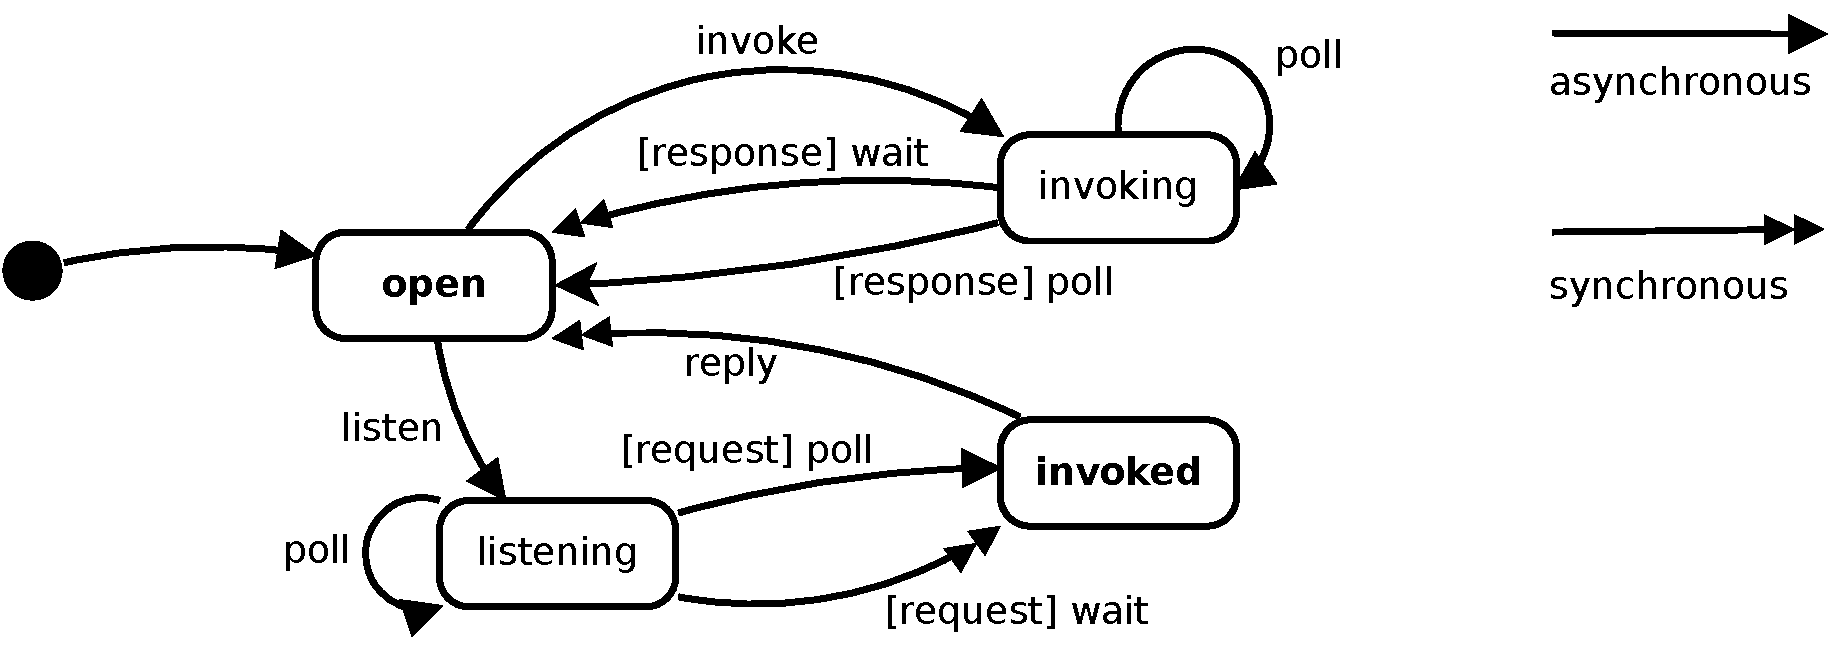
\includegraphics[scale=0.25]{fig/portal.pdf}
\caption{User-visible states of the Portal object.}
\label{fig:portal:state}
\end{center}
\end{figure}

Figure~\ref{fig:portal:state} shows the Portal's states and transitions. Initially, the Portal is in the \emph{open} state and can be configured to either listen for incoming requests or to send a request in the form of an invocation message. The Portal returns to the \emph{open} state by sending a reply in the \emph{invoked} state or by receiving a reply from the \emph{invoked} state. The \emph{invoke}, \emph{listen}, \emph{wait}, and \emph{reply} transitions are triggered through system calls of the Portal's owner. The synchronous transitions return from the system call after the operation completed whereas the asynchronous variants return immediately. 

The message data is stored in an \emph{invocation buffer}, which is shared memory between the application and the Portal on the kernel side. Applications should write to the invocation buffer only when the Portal is in the \emph{open} or \emph{invoked} state. However, this is not enforced by the operating system because non-conforming applications would just interfere with their own operation. The kernel objects that read from the invocation buffer first copy the needed values before checking their validity. Hence, concurrent manipulation of the invocation buffer is ignored.

The following system calls directly interact with the owner's Portal. For convenience and in order to reduce the number of system calls, combined system calls such as \emph{invoke+wait} are available.

\begin{description}
\item[invoke(portal, uctx, dest):] the content of the invocation buffer is sent asynchronously as an invocation to the specific destination \texttt{dest}, which is a capability pointer into the caller's capability space. In general, any kernel object that implement the invoke operation is a valid destination. When used for communication between applications, the destination will be a Portal. The \emph{user context} \texttt{uctx} is an opaque pointer (64bit integer) that is returned by \texttt{wait()} and \texttt{poll()} on arrival of the reply. It is used by the user-space runtime environment to associate received messages with the respective communication channel.
 
\item[listen(portal,uctx):] this asynchronous operation switches the portal to receive mode and allows the Portal to write into the invocation buffer. Otherwise, only the application is allowed to write. Again, the user context \texttt{uctx} is returned by \texttt{wait()} and \texttt{poll()} when a request was received.

\item[reply(portal):] is a synchronous operation that returns after the invocation buffer is copied into the other side's invocation buffer. The operation will succeed quickly because the other side has to wait for the reply already. If the other side's Portal is not ready to receive the response or does no longer exist, the reply operation fails immediately. This ensures that misbehaving clients cannot delay the supervisor's control flows.

\item[bind(portal,ec):] rebinds the Portal to a different Execution Context, which will receive future invocation and reply messages of the Portal. This operation can be issued in any state and just selects the Execution Context that will be resumed by incoming messages. There is a race between rebinding and receiving a message. Whichever is processed first decides which Execution Context handles the message. However, applications that perform rebind in such a receiving state should be prepared to handle the message in both Execution Contexts anyway.   

\item[wait()$\rightarrow$uctx:] is a synchronous operation that blocks until a message on any Portal bound the Execution Context has arrived. The message can be either a invocation or a reply, and may has been arrived on any portal that is in the \emph{listening} or \emph{invoking} state. The user context \texttt{uctx} of the respective \texttt{listen()} and \texttt{invoke()} calls is returned. The \texttt{wait()} call can be interrupted without receiving any message. In that case the value 0 is returned as user context and the error number is set.

\item[poll()$\rightarrow$uctx:] works like \texttt{wait()} but returns immediately if no received messages were pending.
\end{description}

The combination \texttt{invoke+wait} is synchronous and returns when any message was received on one of the execution context's Portals. In contrast, \texttt{invoke+poll} is asynchronous and returns immediately. If a received message was pending in one of the Portals, the respective user context value is returned.


%%%%%%%%%%%%%%%%%%%%%%%%%%%%%%%%%%%%%%%%%%%%%%%%%%%%%%%%%%%%%%%%%%%%%%
\section{Implementation View}
\label{sec:global-development-view}

This section describes implementation aspects, for example, the files and folders structure and the configuration management via code modules.

\subsection{Compile- and Run-Time Dependency Injection}
\label{sec:dependency-injection-impl}

% problem statement
Whenever objects or software components are created by instantiating classes, the question arises how the new objects will interact with the outside world. They require connections to other used services and usually also some context-dependent configuration. These dependencies can be fulfilled by queries to omnipresent directory services, by conventions, or via configuration methods and constructor arguments. 

% our solution
In order to simplify all aspects of instantiation, \mythos applies the principle of \emph{dependency injection} throughout all levels of the architecture and source code. This implies that no object or software component shall search on its own for its dependencies through global variables or omnipresent directory services. Instead, all dependencies and configuration is injected by the creator through constructor arguments and dedicated configuration methods.

This strategy separates the code responsible for instantiation and configuration from the
component's implementation. This helps to reduce the component's assumptions about its usage environment and protects against premature policy decisions.

\begin{description}
\item[Run-time value injection:]
During object creation, the creator passes pointers to used objects and configuration data by value via constructor arguments and additional configuration methods. This is the most commonly used form of dependency injection.

\item[Compile-time template injection:]
In C++, objects are created by instantiating classes and generic class definitions expose template arguments that need to be filled with actual type names and constants. This provides a mechanism for a template type based dependency injection. For example, in order to remove the overhead of virtual methods, the types of used objects can be injected alongside with the pointers to these used objects. This strategy is applied wherever type polymorphism is needed only for configuration but not during the actual execution. 

\item[Compile-time code injection:]
\marginnote{See also~\ref{sec:code-modules-impl}}
Some definitions and constants cannot be injected via template arguments and, sometimes, overuse of template arguments impedes the readability just a bit too much. In these situations, static code injection is applied by including generic header files that will provide the missing definitions. The build configuration management has to supply actual contents for these header files.
\end{description}


\subsection{Source Code Composition: Code Modules}
\label{sec:code-modules-impl}

% problem statement
Earlier work with \mythos showed that a single runtime-only configuration strategy is not sufficient. Some components depend on specific hardware and compiler support, some performance critical options require a static compile-time configuration. At the same time, subtle differences between various platforms (xeonphi, quemu, bochs, gem5\ldots) and the desire to evaluate implementation variants required the ability to replace and recombine code fragments.

% our solution
% source files versus modules versus subsystems
\mythos avoids the conditional C preprocessor spaghetti by applying the principle of dependency injection to the source code organisation. Similar to grouping tightly related objects into components, related source files are grouped into \emph{modules}. In this setting, the kernel objects of \mythos are the user-visible components and modules provide the class definitions that are needed to create the objects of these components. 

The build process is configured by the combination of \emph{module specifications} and a \emph{target specification}. Basically, each module provides a set of source files and requires a set of files. For example, such dependencies can be header files with type definitions or source files with a specific implementation variant of a global function. Most dependencies are extracted automatically from the \texttt{\#include} directives in the provided source files. 

The target specification lists a set of requested modules or files. A simple resolution scheme is used to resolve dependencies: a list of missing files is collected from the requested modules and then additional modules are selected one by one if they provide one of the missing files. Two modules conflict when they provide files with the same destination name. In that case the dependency resolution reports an error and the developer has to manually select one of the possible modules by editing the target specification. In order to reduce the tedious work of selecting large groups of related module variants individually, the respective variants depend on a artificial \emph{tag} as resolution filter and the target specification provides this flag. For example, all modules that target the XeonPhi depend on \texttt{platform:knc} and all modules specific for the x86-64 architecture depend on \texttt{cpu:x86-64}.

\begin{lstlisting}[float, label=lst:module, caption=An example module specification.]
[module.boot-memory-multiboot]
  requires = ["platform:multiboot"]
  incfiles = ["boot/memory/Stage3Setup.h"]
  kernelfiles = ["boot/memory/Stage3Setup.cc", "boot/memory/Stage3Setup.cc", "boot/memory/Stage3Setup-multiboot.cc"]

[module.boot-memory-gem5]
  requires = ["platform:gem5"]
  incfiles = ["boot/memory/Stage3Setup.h"]
  kernelfiles = ["boot/memory/Stage3Setup.cc", "boot/memory/Stage3Setup.cc", "boot/memory/Stage3Setup-e820.cc"]

[module.boot-memory-knc]
  requires = ["platform:knc"]
  incfiles = ["boot/memory/Stage3Setup.h"]
  kernelfiles = ["boot/memory/Stage3Setup.cc", "boot/memory/Stage3Setup.cc", "boot/memory/Stage3Setup-sfi.cc", "boot/memory/Stage3Setup-knc.cc"]
\end{lstlisting}

Listing~\ref{lst:module} shows three example modules that provide the same header file \texttt{Stage3Setup.h} together with with different implementation source files. Instead of selecting one of the variants explicitly, build target specifications declare that they provide one of the platform tags, for example \texttt{platform:knc}. Then, just a single variant has all dependencies fulfilled and will be selected automatically to fulfil the boot codes dependency on \texttt{Stage3Setup.h}.

With respect to the layout of files and folders, modules are grouped into folders based on their respective subsystem with one sub-folder per module. These module folders contain a \texttt{modules.mcconf} file or several \texttt{.conf} files containing module specifications. The pathes to source files are relative to the position of the module specification. The target specifications contains a relative path to the root of the module folders.

The top level source folder structure is roughly based on the horizontal layers. The folder name \texttt{tag} is reserved for \emph{tags}, a symbolic requirements do not refer to a file and is used to specify a configuration without the need to manually pick each platform-dependent module.

The modules folder structure mirrors the structure of the source folder. Each module lives in its own subfolder, shared code is extracted into modules with the suffix ``-common''. There is an additional \emph{build} folder that contains modules facilitating the build process, for example by adding appropriate compiler flags to the makefile.

\subsection{Interacting Asynchronous Objects via Tasklets}
\label{sec:tasklet-impl}

% problem statement
The asynchronous objects' responsibility is to implement delayed and delegated execution as base mechanism for the kernel's concurrency and locality control. Main challenges for any asynchronous execution are the encoding and decoding of the desired action into messages, the storage and transfer of these messages, and the storage of the dynamic processing state.     

% our solution

\begin{lstlisting}[float, label=lst:async-object, caption=An example asynchronous object.]
class Adder {
public:
  void add(Tasklet* msg, AdderResponses* res, int a, int b) {
    monitor.exclusive(msg, [=](Tasklet* msg){this->addImpl(msg,res,a,b);} );
  }

private:
  MutexMonitor monitor;

  void addImpl(Tasklet* msg, AdderResponses* res, int a, int b) {
    // do something ... then respond
    res->addResult(msg, a+b);
    monitor.release();
  }
};
\end{lstlisting}

Listing~\ref{lst:async-object} shows an example implementation of an asynchronous object. The \texttt{Adder} provides the asynchronous method \texttt{Adder::add()} that allows two add two integer numbers.
Given a Tasklet \texttt{msg}, a pointer \texttt{a} to an Adder instance, and a pointer \texttt{r} to a matching response handler object, the asynchronous method is called with \lstinline|a->add(&msg, r, 1000, 1)|. In line 4, the call and its arguments are captured into a C++11 anonymous function (aka closure, lambda expression) and passed to the Adder's monitor (line 4). The monitor uses the passed Tasklet to schedule the delayed and possibly remote execution of the anonymous function. The actual implementation \lstinline|Adder::addImpl()| in line 10 performs its work and, then in line 12, calls one of the result handler's methods, passing along the Tasklet for the asynchronous execution of the handler method. In line 13, the monitor is informed, that the request processing has finished. This is necessary for the asynchronous object deletion. \marginnote{See also~\ref{sec:async-deletion-dyn}}

All execution is non-blocking and, hence, waiting synchronously for results of calls to asynchronous methods is not possible---and not necessary. Instead, \emph{request} methods also retrieve a reference to a response object that acts as continuation and sink for the result data. Such \emph{response} methods consume the tasklet and results as arguments but have no argument pointing to another response handler.

\begin{figure}
  \centering
  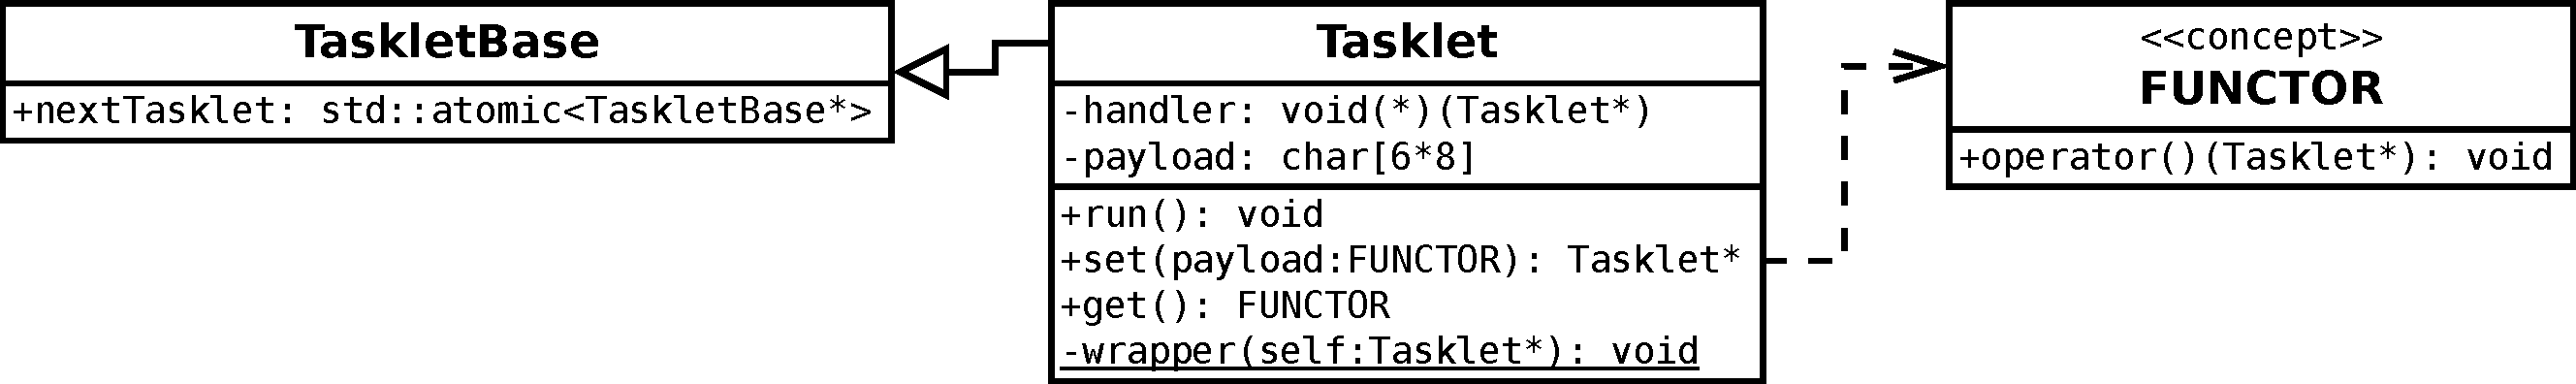
\includegraphics[scale=0.25]{fig/tasklet-class.pdf}
  \caption{Class diagramm of the Tasklet implementation.}
  \label{fig:tasklet-class}
\end{figure}

Figure~\ref{fig:tasklet-class} shows the Tasklet's class diagram. The base class contains an C++11 atomic variable that is used by monitor implementations to manage task queues without dynamic memory management. The pointer is in a separate base class in order to simplify the usage of small dummy objects for the queue management. 

The Tasklet class itself contains a C function pointer very similar to \emph{active messages}. This handler function is responsible for executing the actual function object that was stored through the \lstinline|set()| method in the payload. Instead of the function pointer, a virtual method could have been used. This would consume the same space but adds a second memory lookup via the vtable pointer. The Tasklet implementation contains a generic static implementation for these handler functions.

The size of the payload is chosen such that Tasklets are exactly one x86-64 cacheline large (64 byte). This leaves four 64-bit words for direct call arguments. Any additional arguments have to be passed via a pointer to an argument structure, which is provided by the caller.

\subsection{Managing the Resource Inheritance Tree}
\label{sec:capability-impl}

% problem statement
Storing the complete resource inheritance tree can be very space consuming and most of the information is never used. This reduces the system's efficiency through increased cache and TLB trashing and complicates the concurrent update operations on the inheritance tree. In addition, not all possible inheritance operations have a well-defined meaning. For example, what should happen with the children when a capability that has derived children is copied? Who is responsible for the object deletion when the root capability of an object is copied?

% our solution
\mythos uses a set of rules to restrict the types of capabilities that may be derived to create children and which may be copied to create siblings in the inheritance tree. The basic idea is to maintain a strict \emph{contained-in} relation between the kernel objects and their children. For example, a Portal that was allocated from an Untyped Memory is contained within the address range of the Untyped Memory.

Now, just \emph{references} to kernel objects require separate handling because they represent the same address range as the capability they were derived from. The basic idea is to use a flag in the capability in order to mark it as weak reference. This allows to revoke all references and inform the affected capability subject or object.

However, supervisors may want to transfer access capabilities, which are weak references too, to other applications and retain the option to revoke these individually. For example, a different clients retrieve Portal references to the same portal. In order to keep the different clients apart, these references do not inherit from the original portal but from an intermediate \emph{derived} capability. 
Thus, two flags in the capability are used to represent \emph{original}, \emph{reference}, \emph{derived}, and \emph{reference to derived}. 

\begin{figure}
  \centering
  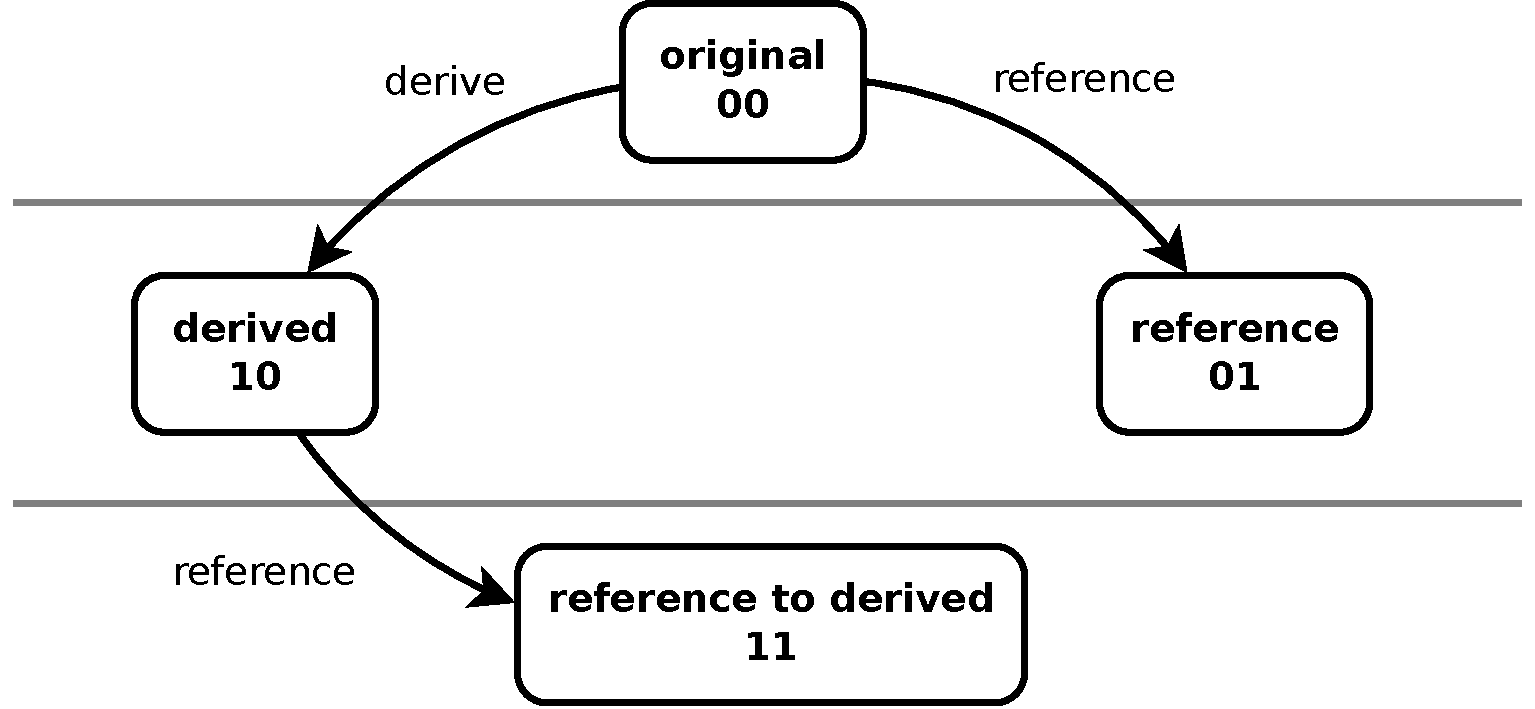
\includegraphics[scale=0.25]{fig/DerivedReferenceBits.pdf}
  \caption{Derivation and reference capability flags. References to derived capabilities can be revoked without revoking other derived capabilities and references to the parent.}
  \label{fig:cap-types}
\end{figure}

This derivation and reference scheme is illustrated in Figure \ref{fig:cap-types}. For example, the original capability can point to a Portal. A reference to the original enables the holder to operate on the Portal as if owns the original. The actual access rights can be restricted through the reference's meta-data. The derived capability of the Portal can be used to hand out derived references to a client application. These can be revoked by revoking the derived capability.  

The same rules are required to differentiate Frames, mapped Frames, derived Frames, and mapped derived Frames. The mapped frames are weak references and are mainly used by the Page Maps to track the usage dependencies between address spaces and frames. The derived frames are used to hand out the right to map frames without loosing the ability to revoke just these mappings.

The above rules have following implications: inheritance from a capability creates a child if the new capability is (a) a reference to an original capability, (b) a reference to a derived capability, (c) a derivation from an original capability, or (d) an original capability that is a real subset of the parent original capability. 
Inheritance creates a sibling in the tree if the new capability is (e) a reference created from a reference, (f) a derivation created from a derivation, or (g) an original capability that has the same address range as its parent capability.
All other cases are prohibited and the rights management may further restrict the inheritance.
% \mythos does not allow the case (g) in order to reduce the amount of reference counting in kernel objects.

\begin{figure}
  \centering
  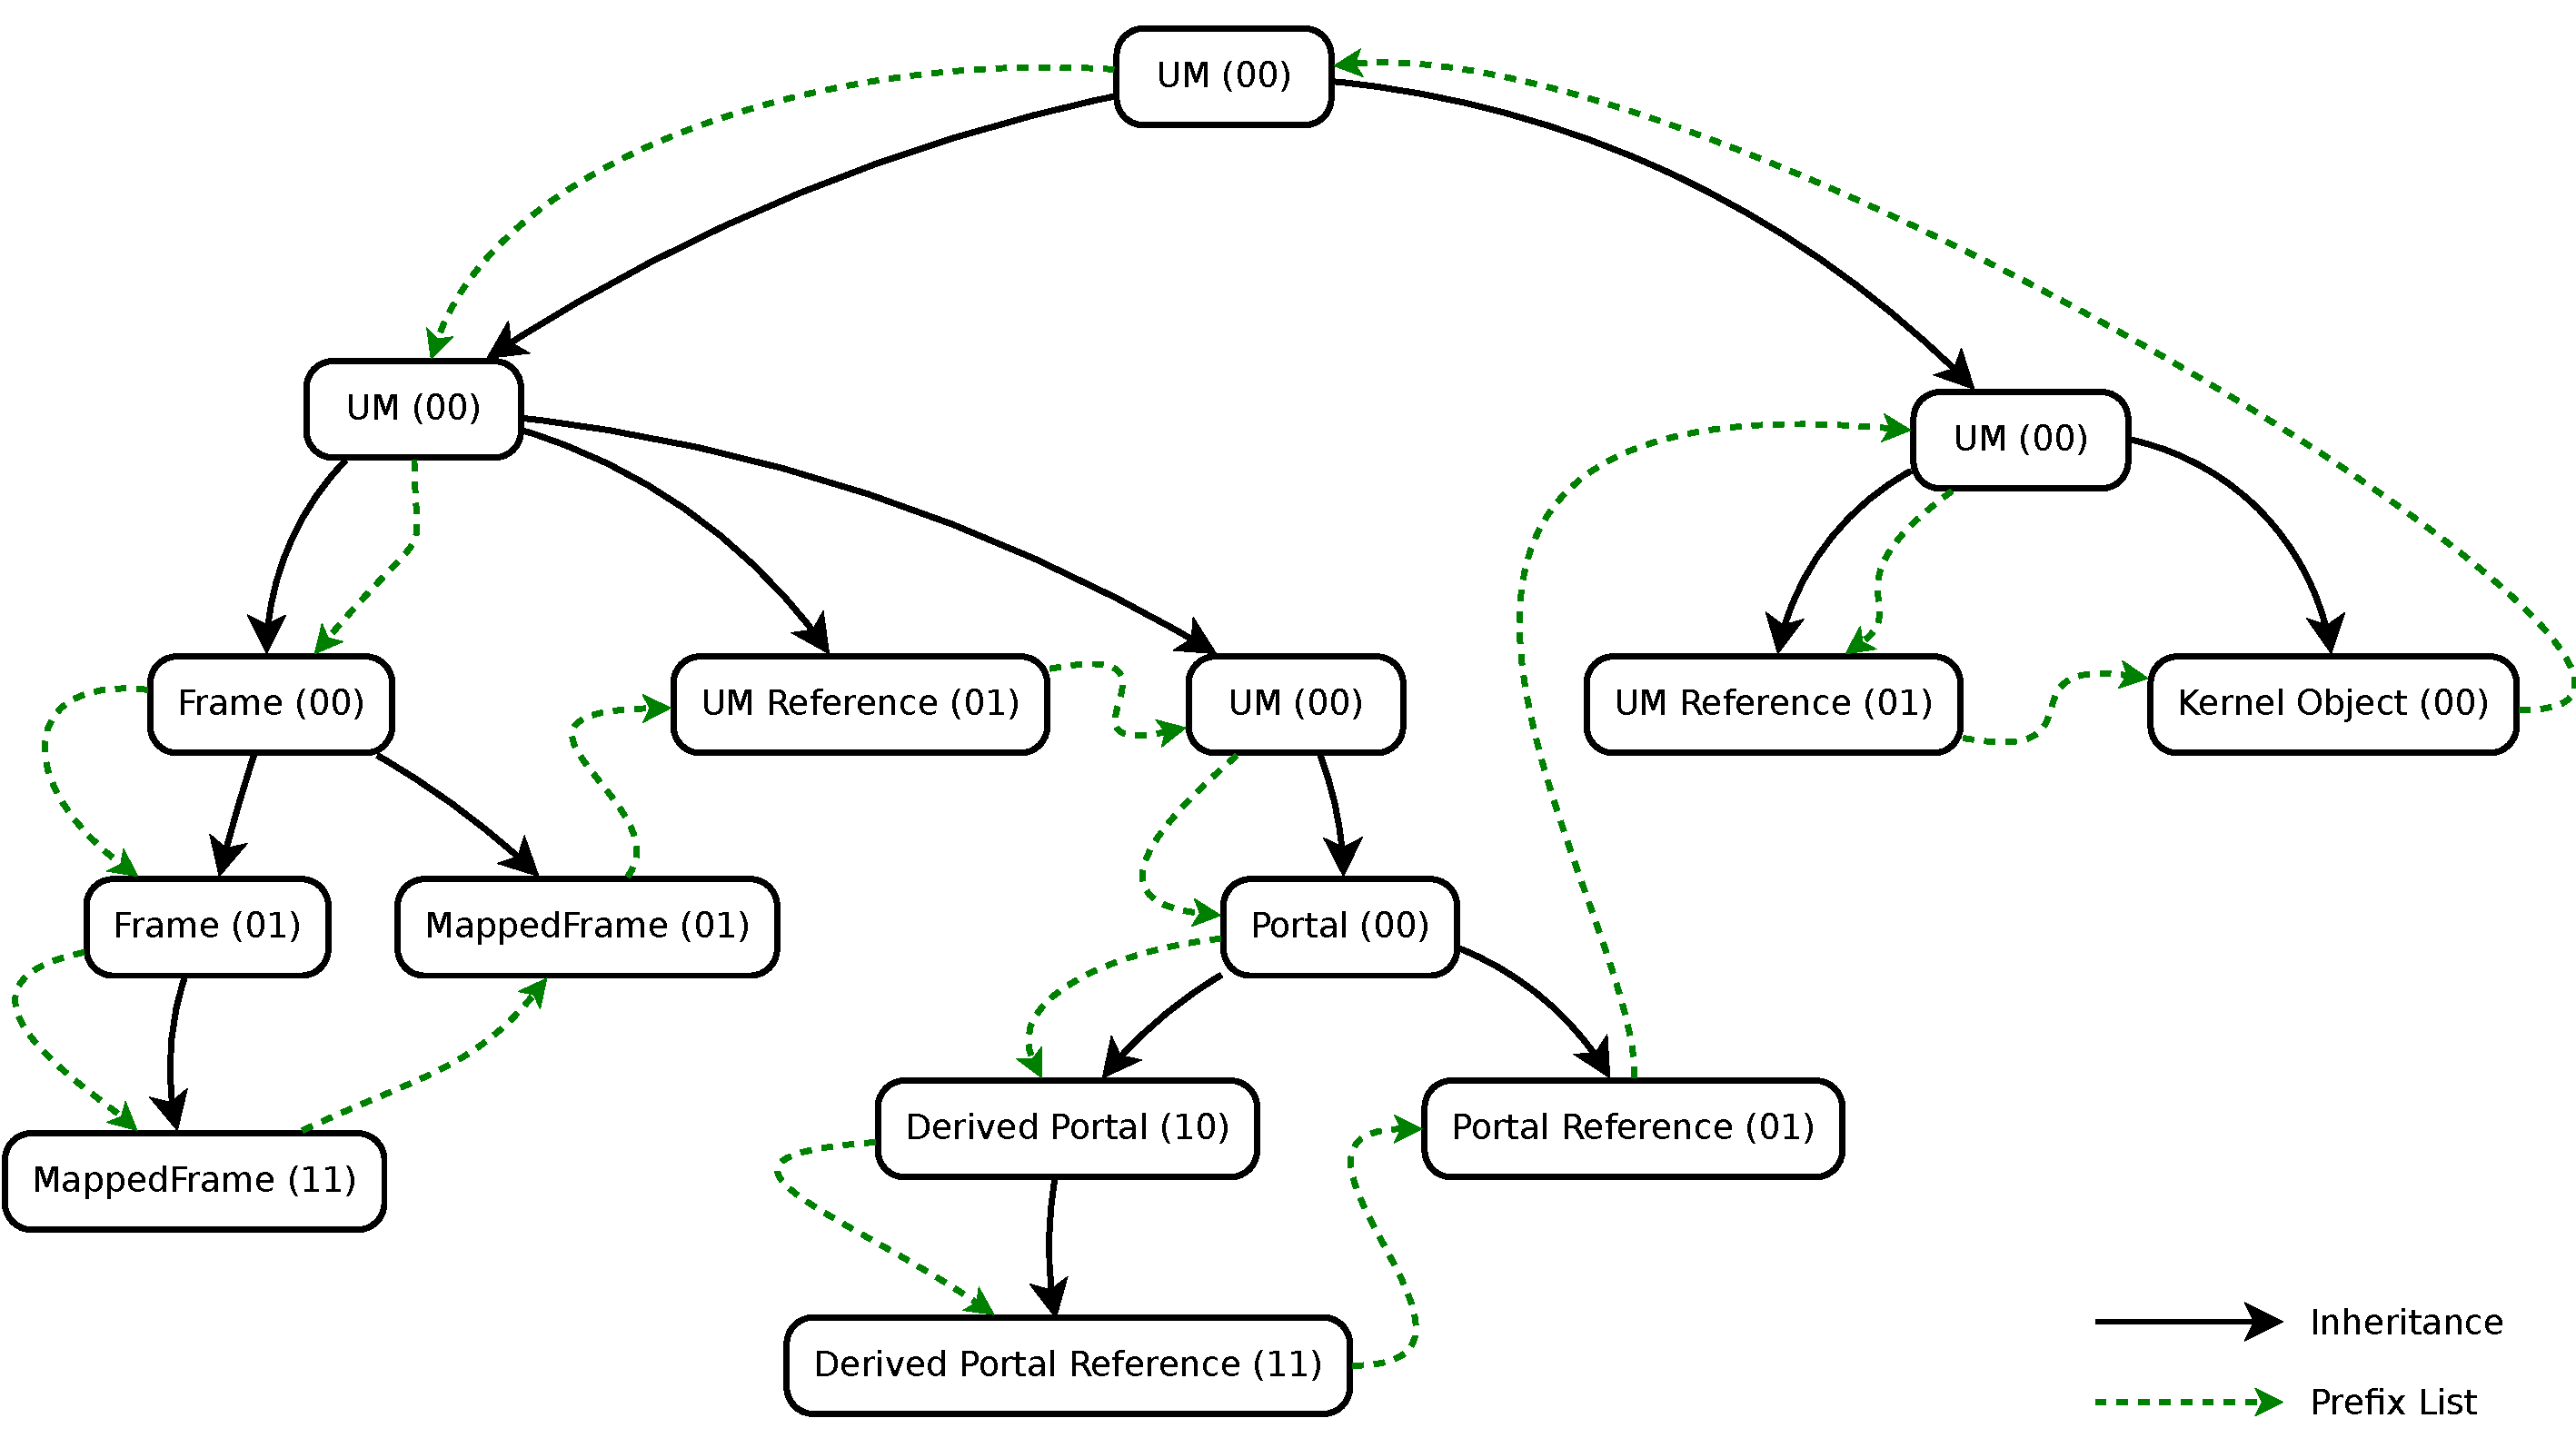
\includegraphics[scale=0.25]{fig/cap-tree.pdf}
  \caption{An example resource inheritance tree. KM is Kernel Memory. The two digits mark original, derivation and reference capabilities. The dotted arrow shows the actually stored prefix serialisation.}
  \label{fig:cap-tree}
\end{figure}

In combination, this allows to store just the \emph{prefix serialisation} of the inheritance tree in a double linked circular list. Figure~\ref{fig:cap-tree} gives an example. The root of the tree is the initial Untyped Memory object that represents all of the kernel's usable memory and is statically owned by the kernel. The circular list avoids to deal with the special case of the list's end. Children are inserted directly behind the parent into this chain. In order to insert a sibling behind a capability, it would be necessary to skip all existing children. Instead, a sibling is inserted before the capability that it inherited from, which equally ensures that both stay within their parent's subtree.

The parent-child relation is not stored explicitly because the objects and properties of the capabilities are sufficient to decide this relation. This is just needed for the revocation of access rights and deletion of kernel objects. By construction, all children are directly behind the parent in the chain. The subtree ends when reaching a capability that cannot be a child of the subtree's root. This \emph{is-child-of} test is successful if (a) the address range owned by the child is a real subset of the parent's range, or their ranges are equal and (b) only the child has the reference flag, or (c) only the child has the derived flag.

\begin{figure}
  \centering
  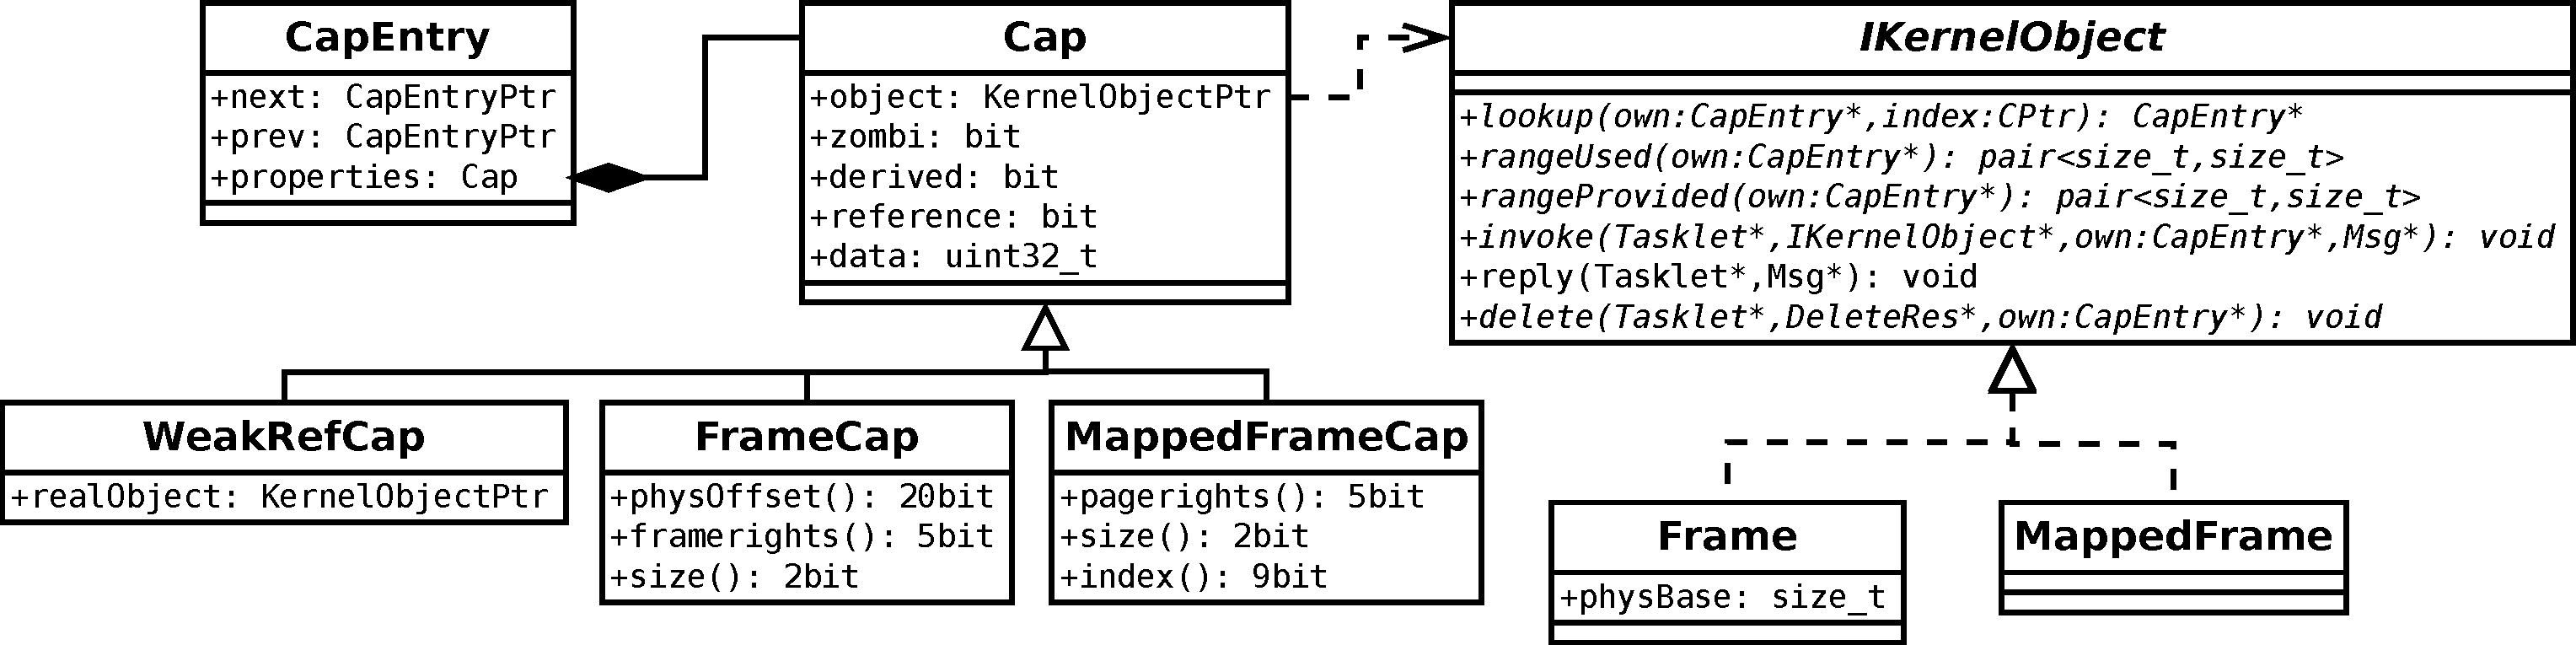
\includegraphics[scale=0.25]{fig/kernel-object-cap.pdf}
  \caption{Class diagram of the prefix-serialised resource inheritance tree.}
  \label{fig:kernel-object-cap}
\end{figure}

Figure~\ref{fig:kernel-object-cap} shows the class diagram of the inheritance tree. The capability entries \texttt{CapEntry} store the double-linked chain and the meta data \texttt{Cap}. The meta data is designed to fit into a 64-bit register. The first 32 bit contain a compressed pointer to the kernel object that is the capability's object. The capability's subject, that is, the holder of the capability entry is not stored by default. The kernel object has to provide the actual information for the inheritance tree management. Most important are \texttt{rangeUsed} and \texttt{rangeProvided} for the \emph{is-child-of} test. The second 32 bit contain arbitrary type-specific meta-data that is processed only by the kernel object. For this purpose, a pointer to the capability entry is passed to all respective methods.

Because of the limited size of the kernel space and the 8-byte alignment of all objects, pointers can be represented with just 29 bits. The remaining three bits are used for status flags such as zombi, derived, and reference. Frames store a 4KiB aligned offset into a 4GiB address window, which requires just 20 bits. The base address of the window is stored in the Frame object.

Weak reference capabilities, for example mapped frames in a page map, require additional consideration. On revocation, the \texttt{delete()} method of the capability's object pointer is called in order to inform the affected kernel object. If this points to the original referenced object, a weak-reference flag and a pointer to the actual subject (the reference holder) is needed in the meta-data. In many cases, it is easier to replace the capability object by a helper kernel object that is part of the subject and knows how to clean up the revoked reference. For example, the object of \texttt{MappedFrameCap} points to a respective kernel object that is part of a \texttt{PageMap}. This leaves more space for other meta-data.

\subsection{Operation Implementation in the Inheritance Tree}
\label{sec:capability-ops} 

Even given the structure of the Inheritance Tree, described in Section \ref{sec:capability-impl}, and the approach to safely delete individual objects, described in Section \ref{sec:async-deletion-dyn}, it is non-trivial to implement high-level operations on Capability considering these operation might be executed parallely.

There are three major categories of operations to consider: The \emph{read operations} read a capability in order to create a reference or call a asynchronous method. The \emph{local operations} locally update the Inheritance Tree, like \emph{derive}, \emph{reference}, but also \emph{moving} a capability into another entry.
The \emph{global operations} consists of operations that may delete whole subtrees of the Inheritance Tree, such as \emph{delete} and \emph{revoke}.

There are several race conditions between operations from different or the same category. The value of a Capability is only updated atomically, and can be marked as a zombie to prevent reader from using the value. A simple solution to resolve the races between writers is protecting the whole Inheritance Tree with a global mutex. However, this serializes all operations which manipulate capabilities.

\begin{figure}
  \centering
  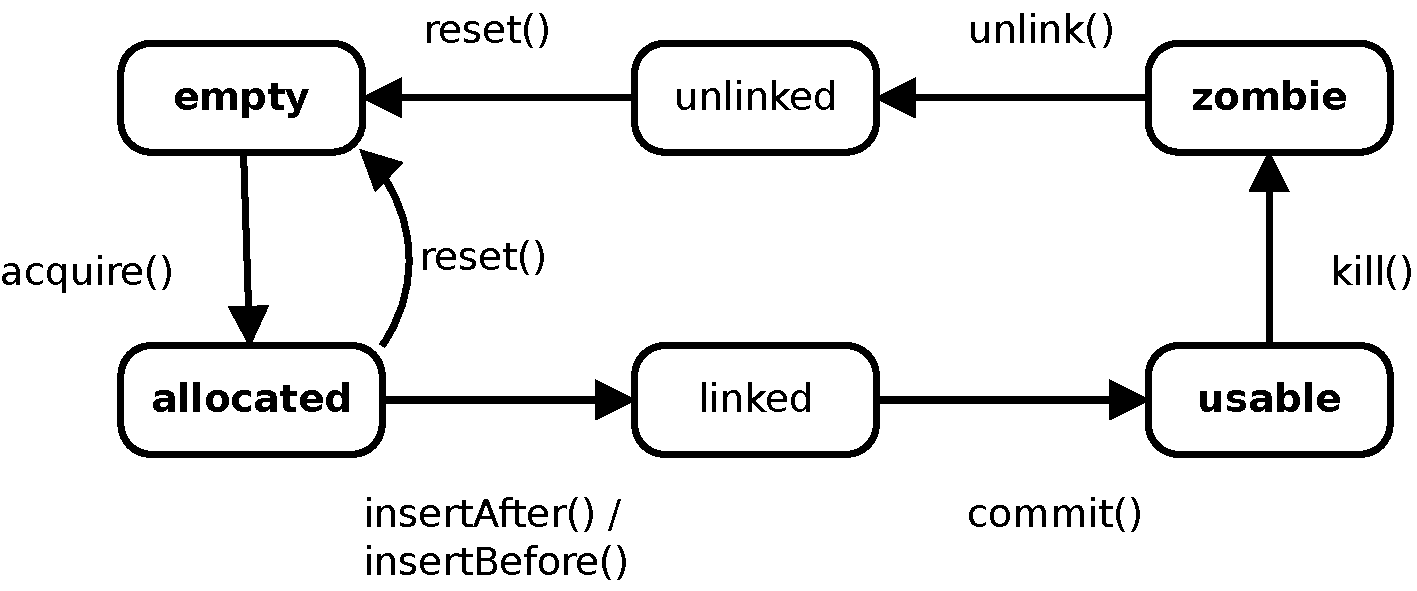
\includegraphics[scale=0.25]{fig/capability-states.pdf}
  \caption{States of the capability object and related operations. State visible from observing only in the capability value are bold.}
  \label{fig:cap-states}
\end{figure}

In order to implement a finer grained locking, individual entries in the inheritance tree (CapEntries) must provide a lock. Similar to the \emph{overhand locking} technique, entries must lock itself and the previous entry in order to be removed. When travesing the list, the lock on the previous entry is release before acquiring the lock on the next entry.

Independant from the locking process, every capability entry has additional states that describe its lifetime cycle, and are illustrated in Figure~\ref{fig:cap-states}:

\begin{description}
\item[empty] In this state, the Capability entry is not linked into the Inheritance Tree, contains no pointer to an object, and has no additional flags set. Such an entry can only be \emph{allocated}.
\item[allocated] After being allocated, the is claimed to be used to store a capability. After allocating the slot, a can try to acquire furter resources, e.g. memory. If that fails, the entry is \emph{reset} into the \emph{empty} state.
\item[linked] This state is the same as the allocated state, but the entry is linked into the tree. After it has been linked, it must be \emph{commited} before the current control flow suspends.
\item[usable] The usable state is the only state in which a subject can access the object through the capability. A usable capability always contains the pointer to a invokable Kernel Object.
\item[zombie] This is a state where the capability still contains the pointer to an kernel object. This enable to revoke the right to access an object immidiately.
\item[unlinked] This state is the same as the zombie state, but the entry is removed from the tree. Unlinking the entry can be used as a sequencer in order to determine who will delete the object.
\end{description}

\emph{Read operations} just load the capability value atomically and check whether the capability is usable, before the pointer value is used to either create a counted reference or issue a request to the object. Races between these requests and delete operations are resolved by the protocol described in Section \ref{sec:async-deletion-dyn}.

\emph{Local operations} manipulate the Inheritance Tree locally and synchronously, thus the can hold locks during the their execution. However, to avoid race conditions with long-running global operations, these local operations must inspect the state of the capability entry and abort if a race is detected. For example, a zombie capability can not be derived nor moved. In order to facilitaty the implementation of the global operations, certain entries can also be pinned to prevent their capabilities from being moved.

\emph{Global operations} potentionally manipulate large portions of the Inheritance Tree and potentionally run for a long time. In order to prevent long-term active waiting, global operations only lock the entrys they are currently manipulating. Races with read or local operations are resolved by setting approbiate flags, such as the zombie flag of the capability or the pinning flag of the entry. Global operation must also take special care to synchronize with each other.

\subsection{Invocation Handling}
\label{sec:invocation-handling}

This section illustrates how Kernel Obects handle invocations and how concurrent application runtimes may expose the invocation to the programmer.
Listing \ref{lst:inv_skel} illustrates invocation handling in the kernel: \emph{invoke} is a ordinary asynchronous function and part of every the Kernel Objects interface. It multiplexes between \emph{different protocols} and invokable \emph{methods} using a \emph{protocol identifier} and a \emph{method identifier}. As most Kernel Objects, the example object only support a single protocol. After the concrete method has been identified, the monitor is requested to execute the implementation of the method. When a method or protocol is requested that is not implemented by the Kernel Object, it immediately returns calls the response handler with a error code.

In the implementation of the invoked method, the invocation message is interpreted further to extract the arguments.
Moreover, the capability is inspected to check if the caller is allowed to invoke the function. If anything fails, the appropriate response \marginnote{See also~\ref{sec:portal-dyn}} is issued. Otherwise, the actual work is done and the context of the invocation is used to return a response according to the protocol. As required for every asynchronous method, the implementation must signal the completion of the request to the monitor.

\begin{lstlisting}[float, label=lst:inv_skel, caption=Kernel-side dispatch and implementation of a method invocation.]
void Adder::invoke(Tasklet* t, InvocationCtx* ctx, CapEntry* cap) {
  switch (ctx->protocol()) {
  case ADDERPROT:
    switch (ctx->method()) {
      case ADD: 
        monitor.request(t, [=](Tasklet*t){this->add(t,ctx,cap)} );
        return;
      }
    break;
  }
  ctx->response(t, CORE, UNKNOWN_METHOD);
}

void Adder::add(Tasklet* t, InvocationCtx* ctx, CapEntry* cap) {
  int a, b;
  bool success = ctx->readMsg(a,b);
  if (!success || !AdderCap(cap).canAdd()) {
  	ctx->response(t, CORE, success ? DENIED : INVALID_MSG); 
  	monitor.requestDone();
  	return;
  }
  // work with ctx->thread(), cap, a, b ...
  ctx->response(t, ADDERPROT, SUM, a+b);
  monitor.requestDone();
}
\end{lstlisting}

Application runtime environments are expected to provide a concurrent programming model, such as coroutines or events. Listing \ref{lst:inv_stub} illustrates how asynchronous invocations can be integrated into an environment which facilitates deferred synchronous execution with \emph{futures}: The invocation is wrapped into a deferred synchronous function that stores its result into a future. Depending on the application-side programming model, the future may trigger an event or reschedule a coroutine when the invocation is completed. Therefore, the application-level idle loop waits for \emph{any} invocation to complete and uses the \emph{user context} \marginnote{See also~\ref{sec:portal-dyn}} in order to dispatch the appropriate response handler. User-level server or services can be implemented analogously: Listening on a Portal also is a deferred synchronous method that returns when a request arrives.

\begin{lstlisting}[float, label=lst:inv_stub, caption=Example for issuing invocation user-side.]
void Adder::add(Portal* p, Future f, int , int b) {
  p->invoke(this->obj, ADDERPROT, ADD, f, a, b); 
}

// ... in app's idle loop:
Portal* res = wait();
if (res) res->handleResponse(); // pushes results to f
\end{lstlisting}

\FloatBarrier
% ------------------------------------------------------------------------------
\selectlanguage{ngerman}
\bibliographystyle{alpha}
\bibliography{literature}

\end{document}
